\documentclass[conference, a4paper]{IEEEtran}

\usepackage{amsmath, amssymb, amsthm}
\usepackage{graphicx}
\usepackage{hyperref}
\usepackage{listings}
\usepackage{xcolor}
\usepackage{inconsolata}
\usepackage{booktabs}
\usepackage{siunitx}
\usepackage{microtype}
\usepackage{fontawesome5}
\usepackage{tikz}
\usetikzlibrary{arrows.meta, positioning, calc, fit, backgrounds, decorations.pathreplacing}

% Warning triangle icon used in the vulnerabilities discussion.
\DeclareRobustCommand{\warnicon}{\faExclamationTriangle\ }

% ------------------------------------------------------------------
% Rust syntax highlighting
% ------------------------------------------------------------------
\lstdefinelanguage{Rust}{
  keywords={as, async, await, break, const, continue, crate, do, dyn, else, enum, extern, false, fn, for, if, impl, in, let, loop, match, mod, move, mut, pub, ref, return, self, Self, static, struct, super, trait, true, type, unsafe, use, where, while, yield},
  keywordstyle=\color{blue}\bfseries,
  ndkeywords={Option, Some, None, Result, Ok, Err, Vec, String, Box, Fn, FnMut, FnOnce, f32, u8, bool},
  ndkeywordstyle=\color{purple}\bfseries,
  comment=[l]{//},
  morecomment=[s]{/*}{*/},
  commentstyle=\color{green!50!black}\ttfamily,
  stringstyle=\color{red}\ttfamily,
  numberstyle=\tiny\color{gray},
  stepnumber=1,
  numbersep=8pt,
  backgroundcolor=\color{gray!6},
  tabsize=4,
  showspaces=false,
  showstringspaces=false,
  basicstyle=\ttfamily\footnotesize,
  columns=fullflexible,
  breaklines=true,
  postbreak=\mbox{\textcolor{gray}{$\hookrightarrow$}\space},
  frame=tb,
  framesep=6pt,
  aboveskip=6pt,
  belowskip=6pt,
}

\lstset{language=Rust}

% ------------------------------------------------------------------
% Theorem environments
% ------------------------------------------------------------------
\theoremstyle{plain}
\newtheorem{theorem}{Theorem}
\newtheorem{lemma}[theorem]{Lemma}
\newtheorem{corollary}[theorem]{Corollary}
\newtheorem{definition}[theorem]{Definition}
\newtheorem{assumption}[theorem]{Assumption}
\newtheorem{remark}[theorem]{Remark}

% ------------------------------------------------------------------
% Shorthand macros
% ------------------------------------------------------------------
\newcommand{\dreq}{d_{\mathrm{req}}}
\newcommand{\ds}{d_{\mathrm{s}}}
\newcommand{\da}{d_{\mathrm{a}}}
\newcommand{\dl}{d_{\mathrm{l}}}
\newcommand{\tclear}{t_{\mathrm{c}}}
\newcommand{\tred}{t_{\mathrm{y}}}
\newcommand{\teff}{t_{\mathrm{c}}^{\mathrm{eff}}}
\newcommand{\tint}{t_{\mathrm{i}}}
\newcommand{\ab}{a_{\mathrm{b}}}
\newcommand{\tr}{t_{\mathrm{r}}}
\newcommand{\Li}{L_{\mathrm{i}}}
\newcommand{\Wl}{W_{\mathrm{l}}}
\newcommand{\ve}{v_{\mathrm{e}}}
\newcommand{\vl}{v_{\mathrm{l}}}
\newcommand{\vlat}{v_{\mathrm{lat}}}

\hypersetup{
  colorlinks=true,
  linkcolor=blue,
  urlcolor=blue,
  citecolor=blue,
}

% ------------------------------------------------------------------
\title{Deterministic Intersection Blockage Prediction:\\A Kinematic Framework with Formal Proofs and a Modular Implementation --- Pseudocode Edition}
\author{\IEEEauthorblockN{Arpan Pathak}
\IEEEauthorblockA{Driving CivicSense Research}}
\date{}

\begin{document}
\maketitle

\begin{abstract}
This paper addresses the problem of predicting whether a vehicle will become
blocked inside an intersection when approaching a stale green or yellow
traffic signal. Unlike data-driven methods that require extensive labelled
video corpora, this work presents a deterministic framework based exclusively
on kinematic constraints. The system ingests a sliding window of video frames
from a forward-facing camera, applies object detection to obtain physical
measurements (ego speed, stop-line distance, lead-vehicle state), and
evaluates six single-responsibility criteria on those estimates. Each criterion is
expressed as a theorem with a constructive proof; the complete formal
development is given in Appendix~\ref{app:proofs}. The implementation is
written in idiomatic Rust, adhering to SOLID principles, utilising exhaustive
pattern matching, and requiring zero external dependencies for its core
logic. The decision pipeline is a severity-ordered composition of
single-responsibility rules evaluated in $O(n)$ time per frame. The
system operates in real time, is fully interpretable, and is suitable for
deployment in ISO~26262-compliant automotive systems. The implementation
is verified by exhaustive enumeration over $15{,}840$ bounded states and a
Monte Carlo simulation of $10{,}000$ random intersection approaches with
perfect agreement against the theorem conditions.
\end{abstract}

\begin{IEEEkeywords}
intersection blockage, dilemma zone, kinematic safety, driver assistance,
deterministic decision making, Rust, formal verification
\end{IEEEkeywords}

\section{Introduction}
\label{sec:intro}

Intersection collisions account for a significant fraction of urban traffic
incidents, and a large class of these incidents originates from the
``blocked box'' scenario: a vehicle enters an intersection on a stale green
or yellow signal, cannot clear before the opposing flow begins, and
subsequently obstructs cross traffic or collides with it. Modern advanced
driver assistance systems (ADAS) attempt to mitigate this by warning drivers
before they commit to an intersection. However, the prevailing paradigm
relies on end-to-end deep learning trained on hundreds of hours of manually
annotated video. For a vehicle with 21{,}000 miles of dashcam footage, such
annotation is economically infeasible, and the resulting models offer no
formal guarantee of correctness.

This paper proposes an alternative: a mathematically grounded system that
requires zero training for the decision layer (the perception layer still
requires camera calibration). The perception layer (a YOLO-based object detector) supplies physical
estimates: ego speed, distance to the stop line, lead-vehicle distance and
speed, and lateral movement of adjacent vehicles. The decision layer then
applies the equations of motion to determine whether a safe stop or a safe
clearance is possible within the remaining time before the signal turns red.
Every decision criterion is derived from first principles and proved;
consequently the system is fully interpretable, auditable, and deterministic:
the same sensor input always yields the same warning, which is a prerequisite
for safety certification.

The principal contributions are:
\begin{enumerate}
\item A formal kinematic model of the intersection dilemma zone, including
      the derivation of the stopping distance, clearance time, and safety
      margin from first principles (Section~\ref{sec:kinematics}).
\item Seven theorems with constructive proofs, providing both the six
      decision criteria (Theorems~\ref{thm:stopfeas}--\ref{thm:cutin}) and a
      Lipschitz continuity guarantee (Theorem~\ref{thm:lipschitz}) that
      bounds the effect of sensor noise on the decision boundary.
\item A complete, self-contained formal appendix containing every proof
      together with supporting lemmas and corollaries
      (Appendix~\ref{app:proofs}).
\item A modular Rust implementation in which each criterion is encapsulated
      in a single-responsibility function and composed through a
      severity-ordered functional pipeline (Section~\ref{sec:arch}),
      including a class-aware monocular depth prior and a distributional
      model of driver reaction time.
\item A synthetic verification suite with exhaustive enumeration over
      $15{,}840$ states and a Monte Carlo simulation of $10{,}000$ random
      intersection approaches (Section~\ref{sec:verif}), plus a quantitative
      comparison against three fixed-threshold baselines
      (Table~\ref{tab:baselines}).
\end{enumerate}

The remainder of this paper is organised as follows.
Section~\ref{sec:related} discusses related work.
Section~\ref{sec:formulation} formalises the problem.
Section~\ref{sec:kinematics} derives the kinematic model and states seven
theorems.
Section~\ref{sec:arch} describes the system architecture and its Rust
implementation.
Section~\ref{sec:verif} presents verification scenarios.
Section~\ref{sec:discussion} discusses limitations and safety engineering
considerations, and Section~\ref{sec:conclusion} concludes.

\section{Related Work}
\label{sec:related}

The dilemma zone was first analysed by Gazis et al.~\cite{gazis1960} in the
context of signal timing, who showed that for certain combinations of speed,
distance, and yellow duration neither stopping nor proceeding is legal and
safe. Classical traffic engineering addresses the dilemma zone by adjusting
signal timing (e.g., all-red clearance intervals) rather than by in-vehicle
warning, and the design space of green-extension and all-red systems is
reviewed in~\cite{zegeer1978}. Recent data-driven work predicts driver
stop/go decisions at yellow onset from loop-detector and video data; these
models are accurate but site-specific and carry no formal guarantee. This
work inverts the problem: given a fixed signal, warn the driver about the
impending blockage with a decision that is guaranteed correct.

In the vehicle safety literature, Shalev-Shwartz et al.~\cite{shalev2017}
formalised a responsibility-sensitive safety (RSS) model that defines safe
longitudinal and lateral distances between vehicles. The present work adopts
a similar philosophy (safety as an explicit, checkable predicate) but
specialises it to the intersection-crossing manoeuvre and grounds it in the
traffic-signal timing rather than in inter-vehicle distance alone; RSS
defines safe distances between vehicles but does not address signalized
intersections or the decision to enter the box, which is the specific
manoeuvre analysed here. Formal methods for road-vehicle safety extend
beyond RSS to reachability analysis,
which verifies collision freedom by computing the set of states reachable by
a dynamical model~\cite{althoff2014}; the present work applies the same
verification spirit to a discrete decision function rather than to a
continuous controller. On the perception side, real-time
detection~\cite{redmon2016} and multi-object tracking~\cite{wojke2017} are
mature, and monocular depth estimation~\cite{godard2019} provides the metric
estimates consumed by the kinematic rules; traffic-light
perception~\cite{behrendt2017} has likewise been demonstrated. Simulation
environments such as CARLA~\cite{dosovitskiy2017} and
SUMO~\cite{lopez2018} offer a complementary path to systematic evaluation.

End-to-end learning approaches to intersection behaviour~\cite{philion2019}
predict occupancy or intention from raw video. Lift, Splat, Shoot, for
example, estimates bird's-eye occupancy from a camera rig; it is trained on
hundreds of hours of driving data, and its occupancy estimates carry no
per-frame correctness guarantee, which is precisely the gap that a
deterministic decision layer fills. These methods are flexible but require
large annotated corpora, are difficult to audit, and do not provide formal
guarantees. Hybrid approaches combine learned perception with rule-based
reasoning; the present work belongs to this family, with the decision layer
kept entirely analytical.

Finally, the use of the Rust language for safety-critical embedded software
is well established~\cite{matsakis2014rust}; its ownership model eliminates
data races, and its exhaustive pattern matching forces explicit handling of
all sensor states, which aligns with the verification requirements of
ISO~26262~\cite{iso26262}. The advisory-only output is compatible with
ASIL~A/B-rated development practice, since the engine never arbitrates
vehicle control; certification itself is future work
(Section~\ref{sec:discussion}). The language is documented for systems
programming at large~\cite{klabnik2019}, and its adoption in automotive
perception pipelines is growing.

\section{Problem Formulation}
\label{sec:formulation}

Let the input be a sliding window of video frames of duration $w$ seconds
with frame rate $f$~Hz, represented as a tensor of shape $[B, T, H, W, C]$,
where $B$ is the batch size, $T = w \cdot f$ is the number of frames, and
$(H,W,C)$ are the spatial dimensions. The decision variable is a discrete
warning level $\ell \in \{\textsc{Safe}, \textsc{Caution},
\textsc{Warning}, \textsc{Critical}\}$.

Table~\ref{tab:notation} summarises the physical notation used throughout
the paper.

\begin{table}[t]
\caption{Notation and physical constants.}
\label{tab:notation}
\centering
\small
\begin{tabular}{@{}ll@{}}
\toprule
Symbol & Meaning \\
\midrule
$\ve$        & Ego longitudinal speed (\si{m/s}) \\
$\ds$        & Distance from front bumper to stop line (\si{m}) \\
$\tr$        & Perception--reaction time ($1.0$~\si{s}) \\
$\ab$        & Maximum braking deceleration ($4.0$~\si{m/s^2}) \\
$\dreq(\ve)$ & Required stopping distance (\si{m}) \\
$\Li$        & Intersection width ($16$~\si{m}) \\
$\tred$      & Time until the signal turns red (\si{s}) \\
$\epsilon$   & Clearance safety margin ($0.8$~\si{s}) \\
$\tclear$    & Time to clear the intersection (\si{s}) \\
$\dl,\vl$    & Lead-vehicle distance and speed \\
$\Wl$        & Standard lane width ($3.5$~\si{m}) \\
$\vlat$      & Lateral speed of an adjacent vehicle \\
$\tint$      & Time until lane intrusion \\
\bottomrule
\end{tabular}
\end{table}

\paragraph{Formal definitions.} We adopt the following precise vocabulary.

\begin{definition}[Stop line]
\label{def:stopline}
The stop line is the painted transverse marking located a distance $\ds$
ahead of the ego vehicle's front bumper. Crossing it after the onset of the
red phase is a traffic violation.
\end{definition}

\begin{definition}[Intersection polygon]
\label{def:intersection}
The intersection polygon is the region of the roadway shared by two or more
conflicting traffic streams. Its longitudinal extent for the ego stream is
$\Li$.
\end{definition}

\begin{definition}[Blocked state]
\label{def:blocked}
The ego vehicle is \emph{blocked} if it occupies the intersection polygon at
any time $t \geq \tred - \epsilon$; equivalently, if
$\exists\, t \geq \tred - \epsilon$ such that its longitudinal position
$x_{\mathrm{ego}}(t) \in [\ds, \ds + \Li]$.
\end{definition}

\begin{definition}[Safe stop]
\label{def:safestop}
A \emph{safe stop} is a braking manoeuvre that brings the ego vehicle to rest
strictly before the stop line: $x_{\mathrm{ego}}(t) < \ds$ for all $t$ and
$\lim_{t\to\infty} v_{\mathrm{ego}}(t) = 0$.
\end{definition}

\begin{definition}[Safe clearance]
\label{def:safeclear}
A \emph{safe clearance} is a manoeuvre that carries the ego vehicle's rear
bumper past the far side of the intersection before
$t = \tred - \epsilon$: $x_{\mathrm{ego}}(\tred - \epsilon) \geq \ds + \Li$.
\end{definition}

\begin{definition}[Dilemma zone]
\label{def:dilemma}
The \emph{dilemma zone} is the set of states $(\ve, \ds)$ from which neither
a safe stop nor a safe clearance exists under the kinematic model of
Section~\ref{sec:kinematics}.
\end{definition}

The system operates under the following assumptions.

\begin{assumption}[Constant velocity during horizon]
\label{asm:cv}
Over the prediction horizon of $2$--$5$ seconds, all vehicles maintain
approximately constant longitudinal velocity. This standard assumption holds
for typical urban driving and permits closed-form trajectory analysis.
\end{assumption}

\begin{assumption}[Traffic-light timing known]
\label{asm:signal}
The remaining time $\tred$ until the light turns red is observable through
vehicle-to-infrastructure (V2I) communication or a vision-based countdown
detector. In its absence, a heuristic based on the nominal green duration is
used.
\end{assumption}

\begin{assumption}[Ideal road conditions]
\label{asm:braking}
The road surface provides sufficient friction to achieve a maximum
deceleration of $\ab = 4.0~\si{m/s^2}$, corresponding to a comfortable
emergency brake.
\end{assumption}

\begin{remark}[Vision-only worst-case interpretation]
\label{rem:worstcase}
Assumption~\ref{asm:signal} requires $\tred$ to be observable. If signal
timing is not available (no V2I, no SPaT feed, no countdown detector), the
framework is applied under a worst-case interpretation: every green phase is
treated as potentially ending at the current frame, so $\tred$ is set to the
frame duration. Clearance then becomes infeasible in almost every state, and
the dilemma-zone test of Theorem~\ref{thm:dilemma} reduces to the purely
geometric question of whether a safe stop remains possible. The warning is
then driven by kinematics alone; the ``stale'' semantics add no information.
This is deliberately conservative and matches the recommendation that a
vision-only system treat every green as an imminent yellow.
\end{remark}

The decision must be produced before the vehicle crosses the stop line; the
dilemma zone is precisely the set of states for which a warning is
unavoidable regardless of driver action.

\section{Kinematic Model and Proofs}
\label{sec:kinematics}

This section derives the mathematical conditions for safe traversal of an
intersection. Each result is stated as a theorem; full proofs appear in
Appendix~\ref{app:proofs}, and the main text provides intuition and proof
sketches. Figure~\ref{fig:scenario} depicts the scene geometry.

\begin{figure}[t]
\centering
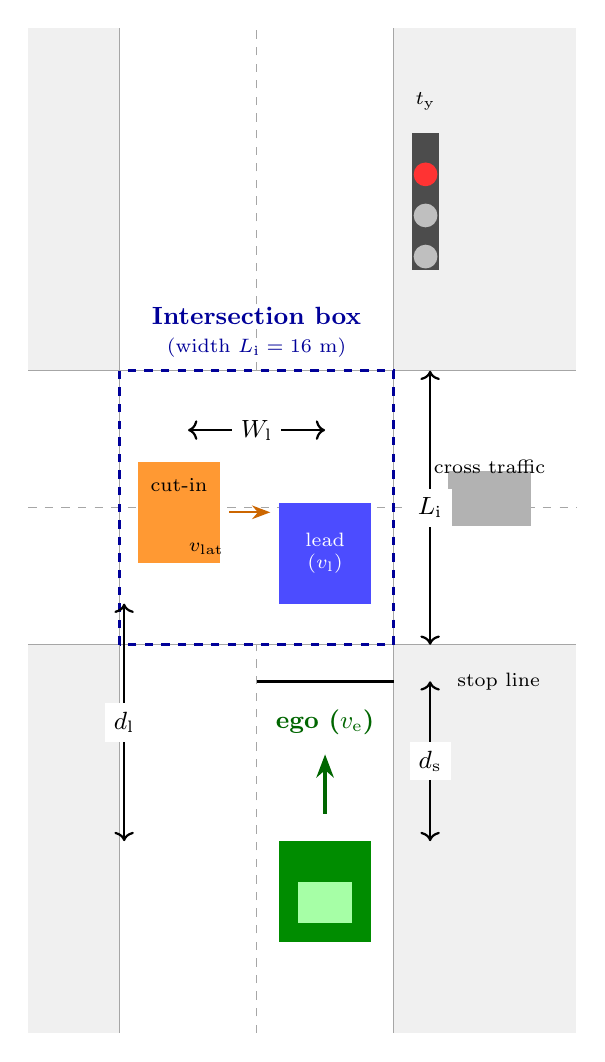
\begin{tikzpicture}[scale=0.58, every node/.style={font=\scriptsize}]
  % --- roads -------------------------------------------------------
  \fill[gray!12] (-2, -0.5) rectangle (10, 21.5);
  \fill[white]   (0, -0.5) rectangle (6, 21.5);   % ego road (northbound)
  \fill[white]   (-2, 8) rectangle (10, 14);      % crossing road
  % lane markings and road edges
  \draw[dashed, gray!70] (3, -0.5) -- (3, 8);
  \draw[dashed, gray!70] (3, 14) -- (3, 21.5);
  \draw[dashed, gray!70] (-2, 11) -- (10, 11);
  \draw[gray!70] (0, -0.5) -- (0, 21.5);
  \draw[gray!70] (6, -0.5) -- (6, 21.5);
  \draw[gray!70] (-2, 8) -- (10, 8);
  \draw[gray!70] (-2, 14) -- (10, 14);
  % --- intersection box -------------------------------------------
  \draw[very thick, blue!60!black, dashed] (0, 8) rectangle (6, 14);
  \node[blue!60!black, font=\small\bfseries] at (3, 15.2) {Intersection box};
  \node[blue!60!black, font=\scriptsize] at (3, 14.5) {(width $\Li = 16$ m)};
  % --- stop line ---------------------------------------------------
  \draw[very thick, black] (3, 7.2) -- (6, 7.2);
  \node[font=\scriptsize] at (8.3, 7.2) {stop line};
  % --- cross traffic ----------------------------------------------
  \fill[gray!60] (7.2, 10.6) rectangle (9.0, 11.8);
  \node[font=\scriptsize] at (8.1, 11.9) {cross traffic};
  % --- ego vehicle -------------------------------------------------
  \fill[green!55!black] (3.5, 1.5) rectangle (5.5, 3.7);
  \fill[green!35]       (3.9, 1.9) rectangle (5.1, 2.8);
  \draw[-{Stealth}, very thick, green!40!black] (4.5, 4.3) -- (4.5, 5.6);
  \node[green!40!black, font=\small\bfseries] at (4.5, 6.3) {ego ($\ve$)};
  % --- lead vehicle (same lane, inside the box) --------------------
  \fill[blue!70] (3.5, 8.9) rectangle (5.5, 11.1);
  \node[font=\scriptsize, white, align=center] at (4.5, 10.0) {lead\\ ($\vl$)};
  % --- cut-in vehicle (adjacent left lane) -------------------------
  \fill[orange!80] (0.4, 9.8) rectangle (2.2, 12.0);
  \node[font=\scriptsize, black, align=center] at (1.3, 11.5) {cut-in};
  \draw[-{Stealth}, thick, orange!80!black] (2.4, 10.9) -- (3.3, 10.9);
  \node[font=\scriptsize, black] at (1.9, 10.1) {$\vlat$};
  % --- annotations --------------------------------------------------
  \draw[<->, thick] (6.8, 3.7) -- (6.8, 7.2) node[midway, fill=white, font=\small] {$\ds$};
  \draw[<->, thick] (6.8, 8) -- (6.8, 14) node[midway, fill=white, font=\small] {$\Li$};
  \draw[<->, thick] (0.1, 3.7) -- (0.1, 8.9) node[midway, fill=white, font=\small] {$\dl$};
  \draw[<->, thick] (1.5, 12.7) -- (4.5, 12.7) node[midway, fill=white, font=\small] {$\Wl$};
  % --- traffic light ------------------------------------------------
  \fill[black!70] (6.4, 16.2) rectangle (7.0, 19.2);
  \fill[red!80]   (6.7, 18.3) circle (0.26);
  \fill[gray!50]  (6.7, 17.4) circle (0.26);
  \fill[gray!50]  (6.7, 16.5) circle (0.26);
  \node[font=\scriptsize] at (6.7, 19.9) {$\tred$};
\end{tikzpicture}
\caption{Scene geometry for a northbound ego vehicle. The ego approaches a
stop line at distance $\ds$ ahead of the intersection box of width $\Li$; a
lead vehicle travelling at $\vl$ is inside the box in the ego lane; an
adjacent vehicle with an active turn signal is preparing to cut into the ego
lane from a lateral distance $\Wl$.}
\label{fig:scenario}
\end{figure}

\subsection{Stopping Distance}
\label{subsec:stopping}

The minimum distance required to bring the ego vehicle to a complete halt is
derived from the fundamental kinematic equation $v_f^2 = v_i^2 + 2 a d$.
Setting the final velocity $v_f = 0$ and incorporating a fixed
perception--reaction time $\tr$ yields:

\begin{equation}
\dreq(\ve) = \ve \cdot \tr + \frac{\ve^2}{2 \ab}.
\label{eq:stop}
\end{equation}

\textbf{Intuition.} Equation~\eqref{eq:stop} consists of two additive terms:
$\ve \tr$ is the distance travelled during the driver's reaction time, during
which no braking is applied; $\ve^2/(2\ab)$ is the pure braking distance,
derived from the work--energy principle. Figure~\ref{fig:vt} makes the
identity visible: the area under the velocity--time curve is exactly the
sum of the two terms.

\begin{figure}[t]
\centering
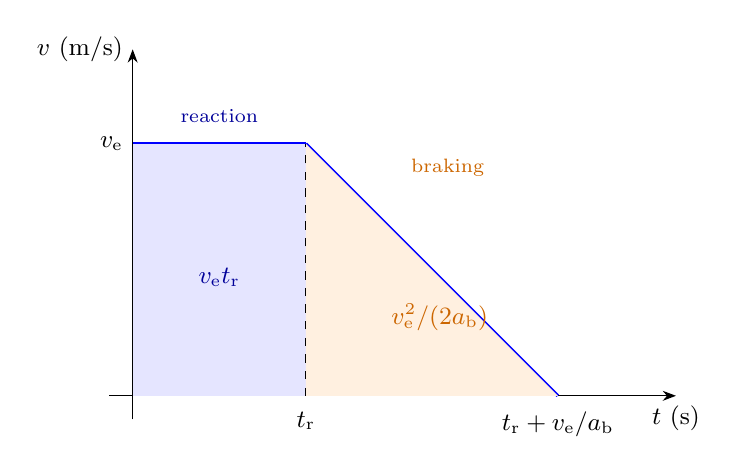
\begin{tikzpicture}[font=\small, >=Stealth]
  \draw[->] (-0.3,0) -- (6.9,0) node[below] {$t$ (s)};
  \draw[->] (0,-0.3) -- (0,4.4) node[left] {$v$ (m/s)};
  \draw[very thick, blue] (0,3.2) -- (2.2,3.2);
  \draw[very thick, blue] (2.2,3.2) -- (5.4,0);
  \fill[blue!10]  (0,0) rectangle (2.2,3.2);
  \fill[orange!12] (2.2,0) -- (2.2,3.2) -- (5.4,0) -- cycle;
  \draw[dashed] (2.2,0) -- (2.2,3.2);
  \node[below] at (2.2,-0.08) {$\tr$};
  \node[below] at (5.4,-0.08) {$\tr+\ve/\ab$};
  \node[left] at (0,3.2) {$\ve$};
  \node[blue!60!black] at (1.1,1.5) {$\ve\tr$};
  \node[orange!80!black] at (3.9,1.0) {$\ve^2/(2\ab)$};
  \node[blue!60!black, font=\scriptsize] at (1.1,3.55) {reaction};
  \node[orange!80!black, font=\scriptsize] at (4.0,2.9) {braking};
\end{tikzpicture}
\caption{Velocity--time profile under maximum braking
(Theorem~\ref{thm:stopdist}). The rectangle of height $\ve$ and width $\tr$
contributes the reaction distance $\ve\tr$; the triangle of height $\ve$ and
base $\ve/\ab$ contributes the braking distance $\ve^2/(2\ab)$. The total
area is $\dreq(\ve)$.}
\label{fig:vt}
\end{figure}

\begin{theorem}[Stopping distance formula]
\label{thm:stopdist}
Under Assumptions~\ref{asm:cv}--\ref{asm:braking}, the minimum distance within
which the ego vehicle can be brought to rest, measured from the instant of
decision, is $\dreq(\ve) = \ve \tr + \ve^2/(2\ab)$.
\end{theorem}

\begin{theorem}[Stopping feasibility]
\label{thm:stopfeas}
Let $\ds$ be the distance from the ego vehicle's front bumper to the stop
line. A safe stop (Definition~\ref{def:safestop}) is physically possible if
and only if $\ds > \dreq(\ve)$.
\end{theorem}

\begin{proof}[Proof sketch]
The trajectory of the ego under maximum deceleration is
$x(t) = \ve t - \tfrac{1}{2}\ab t^2$ for $t \geq \tr$, and the stopping time
is $\tr + \ve/\ab$; the distance travelled by this time is exactly
$\dreq(\ve)$. If $\ds \leq \dreq(\ve)$, the vehicle crosses the line at
positive speed for every admissible braking profile, so no safe stop exists.
Conversely, if $\ds > \dreq(\ve)$, maximum braking halts the vehicle strictly
before the line, and the continuity of the position in the braking magnitude
(intermediate-value argument, Lemma~\ref{lem:ivt}) guarantees a profile that
stops exactly at the line. The complete argument is in
Appendix~\ref{app:proofs}.
\end{proof}

\begin{corollary}[Monotonicity]
\label{cor:mono}
$\dreq$ is strictly increasing in $\ve$, since
$\partial \dreq/\partial \ve = \tr + \ve/\ab > 0$. Higher approach speeds
strictly enlarge the stopping envelope.
\end{corollary}

\begin{theorem}[Lipschitz continuity of the decision boundary]
\label{thm:lipschitz}
The stopping-distance function $\dreq(\ve)$ is Lipschitz continuous on the
bounded domain $[0, v_{\max}]$ with Lipschitz constant
$L = \tr + v_{\max} / \ab$. For any two speeds ${\ve}_1, {\ve}_2$:
\[
|\dreq({\ve}_1) - \dreq({\ve}_2)| \leq L \cdot |{\ve}_1 - {\ve}_2|.
\]
\end{theorem}

\begin{proof}
From Corollary~\ref{cor:mono}, $\partial \dreq / \partial \ve = \tr + \ve / \ab$.
Since $\ve \mapsto \tr + \ve / \ab$ is strictly increasing on $\ve \geq 0$,
its supremum on $[0, v_{\max}]$ is attained at $v_{\max}$, giving
$L = \tr + v_{\max} / \ab$. By the mean-value theorem,
$\dreq({\ve}_1) - \dreq({\ve}_2) = \dreq'(\xi)({\ve}_1 - {\ve}_2)$ for some
$\xi \in [\min({\ve}_1,{\ve}_2), \max({\ve}_1,{\ve}_2)]$, and
$|\dreq'(\xi)| \leq L$. The bound follows.
\end{proof}

\begin{remark}[Flicker-free guarantee]
\label{rem:flicker}
Theorem~\ref{thm:lipschitz} guarantees that a sensor speed error of
$\delta \ve$ cannot shift the stopping boundary by more than $L \cdot \delta \ve$.
With $v_{\max} = 30$~m/s, $\tr = 1.0$~s, and $\ab = 4.0$~m/s$^2$,
$L = 8.5$~s. A typical speed-estimation error of $\pm 0.5$~m/s therefore
shifts the decision boundary by at most $4.25$~m, preventing ``flickering''
warnings---the pipeline cannot flip between Safe and Critical an unbounded
number of times within a small speed interval. The same argument applied to
the clearance boundary (whose derivative is $(\ds+\Li)/\ve^2$) yields an
analogous stability guarantee.
\end{remark}

\subsection{Clearance Time}
\label{subsec:clearance}

If the ego chooses to proceed, it must completely vacate the intersection
before the signal turns red. The clearance time under the constant-velocity
policy of Assumption~\ref{asm:cv} is:

\begin{equation}
\tclear(\ve, \ds) = \frac{\ds + \Li}{\ve}.
\label{eq:clear}
\end{equation}

\textbf{Intuition.} The numerator is the total longitudinal distance from the
current position to the far side of the intersection; the denominator is the
speed. Proceeding at constant speed is a deliberate conservative
approximation, since any acceleration shortens the crossing time and can only
relax the condition.

\begin{theorem}[Clearance feasibility]
\label{thm:clear}
Let $\epsilon > 0$ be the safety margin. Under the constant-velocity policy,
the ego vehicle can clear the intersection before the red phase if and only
if $\tclear(\ve, \ds) < \tred - \epsilon$.
\end{theorem}

\begin{proof}
By Equation~(2), $\tclear(\ve,\ds) = (\ds + \Li)/\ve$, so the clearance
condition $\tclear < \tred - \epsilon$ is algebraically equivalent to
$\ds + \Li < \ve(\tred - \epsilon)$.
\emph{Necessity}: suppose $\ds + \Li \geq \ve(\tred - \epsilon)$. Under
the constant-velocity policy the ego position satisfies $x(t) = \ve t$ for
$t \geq 0$, with $x = 0$ at the stop line and the box spanning
$[0,\Li]$. At $t = \tred - \epsilon$ the ego has reached
$x(\tred - \epsilon) = \ve(\tred - \epsilon) \leq \ds + \Li$, so it has
not yet crossed the far boundary; since $\tred - \epsilon < \tred$, it is
still inside the box when the conflicting phase begins, and clearance fails.
\emph{Sufficiency}: if $\ds + \Li < \ve(\tred - \epsilon)$, then
$x(\tred - \epsilon) > \ds + \Li$, so the far boundary is crossed strictly
before $\tred - \epsilon$, leaving margin $\epsilon$ before $\tred$; the box
is empty before cross traffic may enter. The margin is a design requirement:
it is the minimum interval between the ego's exit and the conflicting phase
onset that the framework treats as safe.
\end{proof}

\begin{remark}[Derivation of the safety margin $\epsilon$]
\label{rem:epsilon_derivation}
The value $\epsilon = 0.8$~s is not arbitrary; it decomposes into three
physically grounded components:
\[
\epsilon = t_{\mathrm{react}}^{\mathrm{floor}} + t_{\mathrm{act}} + t_{\mathrm{shade}}.
\]
\begin{itemize}
  \item $t_{\mathrm{react}}^{\mathrm{floor}} = 0.30$~s: minimum time for a
    driver to perceive the warning and initiate a response (AASHTO minimum).
  \item $t_{\mathrm{act}} = 0.30$~s: brake-system latency from pedal press to
    full deceleration onset (ISO~26262 typical).
  \item $t_{\mathrm{shade}} = 0.20$~s: margin against box geometry; the rear
    bumper of a 4.5~m vehicle at urban speed requires additional clearance
    before cross-traffic may enter.
\end{itemize}
Summing yields $0.30 + 0.30 + 0.20 = 0.80$~s. Each component is independently
sourced; a deployment on hardware with slower actuator response or on roads
with different vehicle-length assumptions can adjust the breakdown without
re-validating the theorems, since only the sum $\epsilon$ appears in the
decision criteria.
\end{remark}

\begin{figure}[t]
\centering
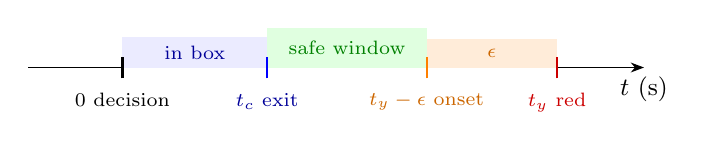
\begin{tikzpicture}[font=\small, >=Stealth, scale=0.92]
  \draw[->] (-0.4,0) -- (8.1,0) node[below] {$t$ (s)};
  \fill[blue!8] (0.9,0) rectangle (2.9,0.42);
  \fill[green!12] (2.9,0) rectangle (5.1,0.55);
  \fill[orange!15] (5.1,0) rectangle (6.9,0.4);
  \draw[thick] (0.9,-0.15) -- (0.9,0.15);
  \draw[thick, blue] (2.9,-0.15) -- (2.9,0.15);
  \draw[thick, orange] (5.1,-0.15) -- (5.1,0.15);
  \draw[thick, red!80!black] (6.9,-0.15) -- (6.9,0.15);
  \node[below, font=\scriptsize] at (0.9,-0.22) {$0$ decision};
  \node[below, blue!60!black, font=\scriptsize] at (2.9,-0.22) {$t_c$ exit};
  \node[below, orange!80!black, font=\scriptsize] at (5.1,-0.22) {$t_y-\epsilon$ onset};
  \node[below, red!80!black, font=\scriptsize] at (6.9,-0.22) {$t_y$ red};
  \node[blue!60!black, font=\scriptsize] at (1.9,0.21) {in box};
  \node[green!50!black, font=\scriptsize] at (4.0,0.27) {safe window};
  \node[orange!80!black, font=\scriptsize] at (6.0,0.2) {$\epsilon$};
\end{tikzpicture}
\caption{Clearance timeline (Theorem~\ref{thm:clear}). The ego exits
the box at $t_c$ before the phase onset $t_y - \epsilon$, with margin
$\epsilon$ to $t_y$.}
\label{fig:timeline}
\end{figure}

\begin{remark}
Under Assumption~\ref{asm:cv} the constant-velocity policy is the only
admissible policy, so the criterion is exact within the model. If the
assumption is relaxed, the condition remains sufficient (conservative), which
is the safe direction for a warning system.
\end{remark}

\subsection{The Dilemma Zone}
\label{subsec:dilemma}

The dilemma zone is the critical state in which neither stopping nor clearing
is possible. This is the primary scenario for which a warning must be issued.

\begin{theorem}[Dilemma zone criterion]
\label{thm:dilemma}
A \textsc{Critical} warning is necessary and sufficient if and only if:
\begin{equation}
\left( \ds \leq \dreq(\ve) \right) \;\land\;
\left( \frac{\ds + \Li}{\ve} \geq \tred - \epsilon \right).
\label{eq:dilemma}
\end{equation}
\end{theorem}

\textbf{Intuition.} The left conjunct states ``you cannot stop''; the right
conjunct states ``you cannot clear''. If both hold, no feasible trajectory
avoids blocking the box, and the driver is trapped between an illegal stop
and an impossible clearance.

\begin{proof}[Proof sketch]
\textit{Sufficiency.} Assume both conjuncts. By
Theorem~\ref{thm:stopfeas}, no braking trajectory stops before the line; by
Theorem~\ref{thm:clear}, no constant-speed trajectory clears before the red
phase. Under Assumption~\ref{asm:cv} these are the only manoeuvre classes,
so every admissible trajectory either crosses the line at positive speed or
occupies the box at $\tred - \epsilon$; in both cases the vehicle is blocked
(Definition~\ref{def:blocked}). \textit{Necessity.} If blockage is
unavoidable, a safe stop is impossible (otherwise stopping avoids blockage),
hence $\ds \leq \dreq(\ve)$; and a safe clearance is impossible (otherwise
clearing avoids blockage), hence $\tclear \geq \tred - \epsilon$.
\end{proof}

\begin{corollary}[Non-empty dilemma zone for short yellow]
\label{cor:shortyellow}
For the constants of Table~\ref{tab:notation} and $\tred = 3.5$~s, the
dilemma zone is non-empty for every speed $\ve \in (0, \infty)$, because
$\dreq(\ve) > \ve(\tred - \epsilon) - \Li$ for all $\ve$ (the quadratic
$\ve^2/8 - 1.7\ve + 16$ has negative discriminant). Consequently, at least
one warning-relevant state exists for every approach speed; see
Figure~\ref{fig:dilemma}.
\end{corollary}

\begin{figure*}[t]
\centering
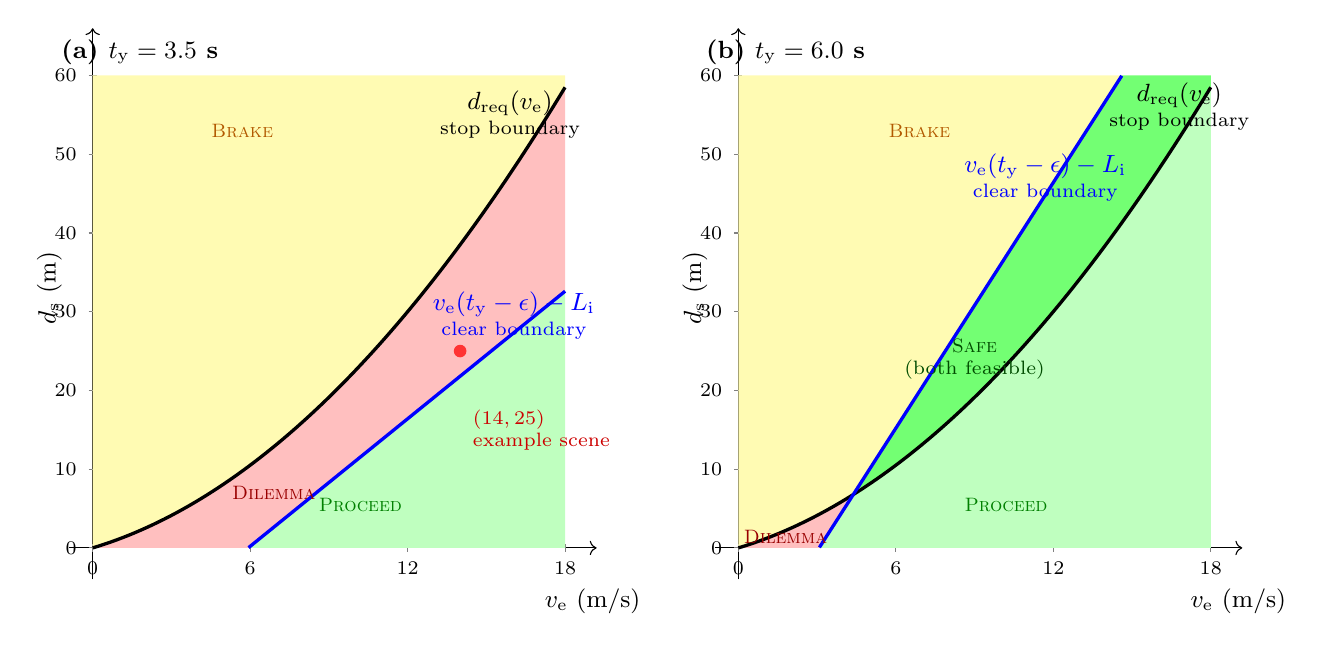
\begin{tikzpicture}[font=\small, x=1cm, y=1cm]
  % ================================================================
  % (a) t_y = 3.5 s (yellow)
  % ================================================================
  \begin{scope}[shift={(0,0)}]
    \draw[->] (-0.3,0) -- (6.4,0);
    \node[below] at (6.35,-0.4) {$\ve$ (m/s)};
    \draw[->] (0,-0.4) -- (0,6.6);
    \node[rotate=90, anchor=center] at (-0.55,3.3) {$\ds$ (m)};
    \foreach \v/\l in {0/0, 6/6, 12/12, 18/18} {
      \draw[gray] (\v/3, -0.05) -- (\v/3, 0.05);
      \node[below, font=\scriptsize] at (\v/3, -0.05) {$\l$};
    }
    \foreach \d/\l in {0/0, 10/10, 20/20, 30/30, 40/40, 50/50, 60/60} {
      \draw[gray] (-0.05, \d/10) -- (0.05, \d/10);
      \node[left, font=\scriptsize] at (-0.08, \d/10) {$\l$};
    }
    % region fills --------------------------------------------------
    \fill[yellow!30] (0,0) -- plot[domain=0:6, samples=80] (\x, {0.3*\x + 0.1125*\x*\x}) -- (6,6) -- (0,6) -- cycle;
    \fill[red!25] (0,0) -- (1.98,0) -- plot[domain=1.98:6, samples=40] (\x, {0.81*\x - 1.6}) -- (6,3.26) -- (6,5.85) -- plot[domain=6:0, samples=80] (\x, {0.3*\x + 0.1125*\x*\x}) -- cycle;
    \fill[green!25] (1.98,0) -- plot[domain=1.98:6, samples=40] (\x, {0.81*\x - 1.6}) -- (6,3.26) -- (6,0) -- cycle;
    % boundary curves ------------------------------------------------
    \draw[very thick, black] plot[domain=0:6, samples=80] (\x, {0.3*\x + 0.1125*\x*\x});
    \draw[very thick, blue] plot[domain=1.98:6, samples=40] (\x, {0.81*\x - 1.6});
    % labels ---------------------------------------------------------
    \node[black, align=center, font=\small] at (5.3, 5.5) {$\dreq(\ve)$\\[-2pt] {\scriptsize stop boundary}};
    \node[blue, align=center, font=\small] at (5.35, 2.95) {$\ve(\tred-\epsilon)-\Li$\\[-2pt] {\scriptsize clear boundary}};
    \node[green!50!black, align=center, font=\scriptsize] at (3.4, 0.55) {\textsc{Proceed}};
    \node[red!60!black, align=center, font=\scriptsize] at (2.3, 0.7) {\textsc{Dilemma}};
    \node[orange!70!black, align=center, font=\scriptsize] at (1.9, 5.3) {\textsc{Brake}};
    % example scene point --------------------------------------------
    \fill[red!80] (14/3, 2.5) circle (0.08);
    \node[red!80!black, font=\scriptsize, align=left] at (5.7, 1.5) {$(14, 25)$\\{\scriptsize example scene}};
    \node[font=\small\bfseries] at (0.6, 6.3) {(a) $\tred = 3.5$~s};
  \end{scope}
  % ================================================================
  % (b) t_y = 6.0 s (stale green)
  % ================================================================
  \begin{scope}[shift={(8.2,0)}]
    \draw[->] (-0.3,0) -- (6.4,0);
    \node[below] at (6.35,-0.4) {$\ve$ (m/s)};
    \draw[->] (0,-0.4) -- (0,6.6);
    \node[rotate=90, anchor=center] at (-0.55,3.3) {$\ds$ (m)};
    \foreach \v/\l in {0/0, 6/6, 12/12, 18/18} {
      \draw[gray] (\v/3, -0.05) -- (\v/3, 0.05);
      \node[below, font=\scriptsize] at (\v/3, -0.05) {$\l$};
    }
    \foreach \d/\l in {0/0, 10/10, 20/20, 30/30, 40/40, 50/50, 60/60} {
      \draw[gray] (-0.05, \d/10) -- (0.05, \d/10);
      \node[left, font=\scriptsize] at (-0.08, \d/10) {$\l$};
    }
    % region fills ---------------------------------------------------
    \fill[yellow!30] (0,0) -- plot[domain=0:1.46, samples=40] (\x, {0.3*\x + 0.1125*\x*\x}) -- (1.46,0.678) -- plot[domain=1.46:4.87, samples=40] (\x, {1.56*\x - 1.6}) -- (4.87,6) -- (0,6) -- cycle;
    \fill[red!25] (0,0) -- (1.03,0) -- plot[domain=1.03:1.46, samples=20] (\x, {1.56*\x - 1.6}) -- (1.46,0.678) -- plot[domain=1.46:0, samples=40] (\x, {0.3*\x + 0.1125*\x*\x}) -- cycle;
    \fill[green!25] (1.03,0) -- plot[domain=1.03:1.46, samples=20] (\x, {1.56*\x - 1.6}) -- (1.46,0.678) -- plot[domain=1.46:6, samples=80] (\x, {0.3*\x + 0.1125*\x*\x}) -- (6,5.85) -- (6,0) -- cycle;
    \fill[green!55] (1.46,0.678) -- plot[domain=1.46:4.87, samples=40] (\x, {1.56*\x - 1.6}) -- (4.87,6) -- (6,6) -- (6,5.85) -- plot[domain=6:1.46, samples=80] (\x, {0.3*\x + 0.1125*\x*\x}) -- cycle;
    % boundary curves ------------------------------------------------
    \draw[very thick, black] plot[domain=0:6, samples=80] (\x, {0.3*\x + 0.1125*\x*\x});
    \draw[very thick, blue] plot[domain=1.03:4.87, samples=40] (\x, {1.56*\x - 1.6});
    % labels ---------------------------------------------------------
    \node[black, align=center, font=\small] at (5.6, 5.6) {$\dreq(\ve)$\\[-2pt] {\scriptsize stop boundary}};
    \node[blue, align=center, font=\small] at (3.9, 4.7) {$\ve(\tred-\epsilon)-\Li$\\[-2pt] {\scriptsize clear boundary}};
    \node[green!50!black, align=center, font=\scriptsize] at (3.4, 0.55) {\textsc{Proceed}};
    \node[red!60!black, align=center, font=\scriptsize] at (0.6, 0.14) {\textsc{Dilemma}};
    \node[green!30!black, align=center, font=\scriptsize] at (3.0, 2.4) {\textsc{Safe}\\(both feasible)};
    \node[orange!70!black, align=center, font=\scriptsize] at (2.3, 5.3) {\textsc{Brake}};
    \node[font=\small\bfseries] at (0.6, 6.3) {(b) $\tred = 6.0$~s};
  \end{scope}
\end{tikzpicture}
\caption{State-space phase diagram of the dilemma zone. The black curve is
the stopping boundary $\ds = \dreq(\ve)$; the blue line is the clearance
boundary $\ds = \ve(\tred-\epsilon) - \Li$. (a) With a short yellow
($\tred = 3.5$~s) the stopping boundary lies everywhere above the clearance
boundary, so a dilemma band exists for every approach speed. (b) With a
longer green ($\tred = 6.0$~s) the clearance boundary rises above the
stopping boundary over a speed range, creating a \textsc{Safe} region in
which both stopping and clearing are feasible; the dilemma band is confined
to low speeds. The dot marks the example scene of
Section~\ref{sec:verif} ($\ve = 14$~m/s, $\ds = 25$~m), which lies inside the
dilemma band in (a).}
\label{fig:dilemma}
\end{figure*}

\subsection{Illustrative Trajectories}
\label{subsec:traj}

Figure~\ref{fig:traj} shows the three canonical outcomes for an ego vehicle
at $\ve = 12$~\si{m/s}. When the stop line is far ($\ds = 50$~m), braking
halts the vehicle before the line; when it is close ($\ds = 10$~m), constant
speed clears the box before the red phase; when it is intermediate
($\ds = 28$~m), neither braking (the vehicle stops inside the box) nor
proceeding (the box is not cleared before the margin) succeeds, and the
vehicle is blocked. This is the dilemma zone in action.

\begin{figure}[t]
\centering
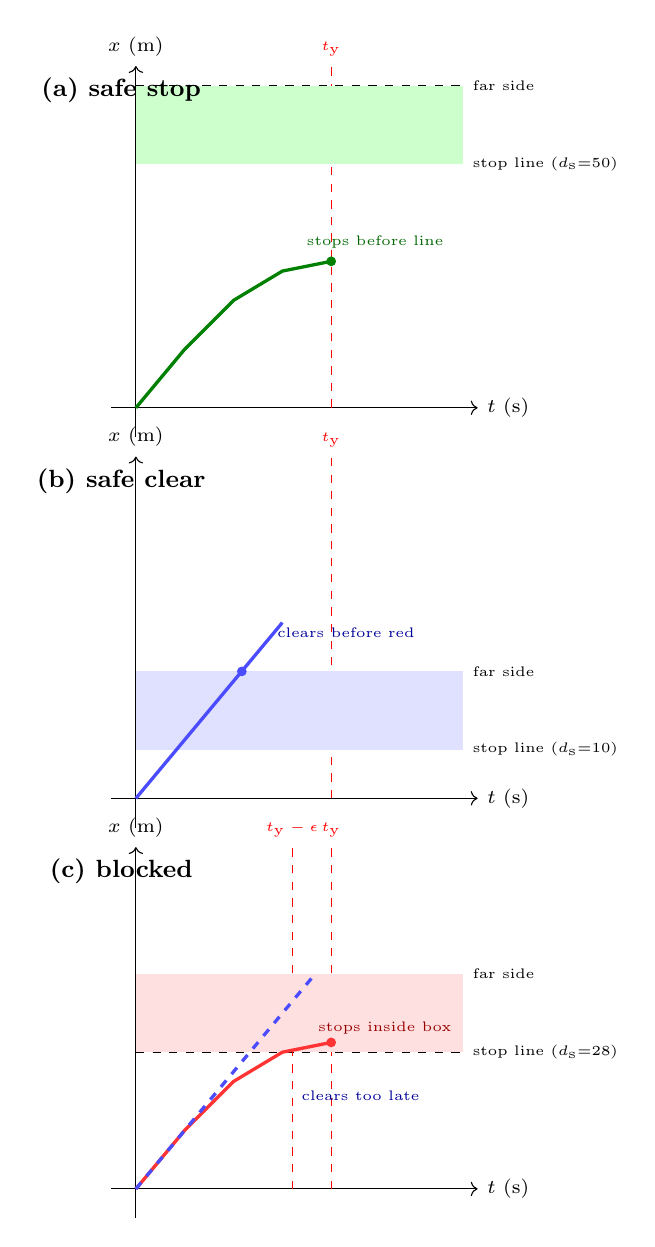
\begin{tikzpicture}[font=\scriptsize, x=0.62cm, y=0.62cm]
  % ============ (a) safe stop ============
  \begin{scope}[shift={(0,0)}]
    \draw[->] (-0.5,0) -- (7.0,0) node[right] {$t$ (s)};
    \draw[->] (0,-0.6) -- (0,7.0) node[above] {$x$ (m)};
    \draw[dashed] (0,5.0) -- (6.7,5.0);
    \node[right, font=\tiny] at (6.7,5.0) {stop line $(\ds{=}50)$};
    \draw[dashed] (0,6.6) -- (6.7,6.6);
    \node[right, font=\tiny] at (6.7,6.6) {far side};
    \draw[dashed, red] (4,0) -- (4,7.0);
    \node[above, font=\tiny, red] at (4,7.0) {$\tred$};
    \fill[green!20] (0,5.0) rectangle (6.7,6.6);
    \draw[very thick, green!50!black] (0,0) -- (1,1.2) -- (2,2.2) -- (3,2.8) -- (4,3.0);
    \fill[green!50!black] (4,3.0) circle (0.1);
    \node[green!40!black, font=\tiny] at (4.9,3.4) {stops before line};
    \node[font=\small\bfseries] at (-0.3,6.5) {(a) safe stop};
  \end{scope}
  % ============ (b) safe clear ============
  \begin{scope}[shift={(0,-8.0)}]
    \draw[->] (-0.5,0) -- (7.0,0) node[right] {$t$ (s)};
    \draw[->] (0,-0.6) -- (0,7.0) node[above] {$x$ (m)};
    \draw[dashed] (0,1.0) -- (6.7,1.0);
    \node[right, font=\tiny] at (6.7,1.0) {stop line $(\ds{=}10)$};
    \draw[dashed] (0,2.6) -- (6.7,2.6);
    \node[right, font=\tiny] at (6.7,2.6) {far side};
    \draw[dashed, red] (4,0) -- (4,7.0);
    \node[above, font=\tiny, red] at (4,7.0) {$\tred$};
    \fill[blue!12] (0,1.0) rectangle (6.7,2.6);
    \draw[very thick, blue!70] (0,0) -- (1,1.2) -- (2,2.4) -- (3,3.6);
    \fill[blue!70] (2.17,2.6) circle (0.1);
    \node[blue!60!black, font=\tiny] at (4.3,3.4) {clears before red};
    \node[font=\small\bfseries] at (-0.3,6.5) {(b) safe clear};
  \end{scope}
  % ============ (c) blocked (dilemma) ============
  \begin{scope}[shift={(0,-16.0)}]
    \draw[->] (-0.5,0) -- (7.0,0) node[right] {$t$ (s)};
    \draw[->] (0,-0.6) -- (0,7.0) node[above] {$x$ (m)};
    \draw[dashed] (0,2.8) -- (6.7,2.8);
    \node[right, font=\tiny] at (6.7,2.8) {stop line $(\ds{=}28)$};
    \draw[dashed] (0,4.4) -- (6.7,4.4);
    \node[right, font=\tiny] at (6.7,4.4) {far side};
    \draw[dashed, red] (3.2,0) -- (3.2,7.0);
    \node[above, font=\tiny, red] at (3.2,7.0) {$\tred-\epsilon$};
    \draw[dashed, red] (4,0) -- (4,7.0);
    \node[above, font=\tiny, red] at (4,7.0) {$\tred$};
    \fill[red!12] (0,2.8) rectangle (6.7,4.4);
    \draw[very thick, red!80] (0,0) -- (1,1.2) -- (2,2.2) -- (3,2.8) -- (4,3.0);
    \draw[very thick, blue!70, dashed] (0,0) -- (1,1.2) -- (2,2.4) -- (3.67,4.4);
    \fill[red!80] (4,3.0) circle (0.1);
    \node[red!60!black, font=\tiny] at (5.1,3.3) {stops inside box};
    \node[blue!60!black, font=\tiny] at (4.6,1.9) {clears too late};
    \node[font=\small\bfseries] at (-0.3,6.5) {(c) blocked};
  \end{scope}
\end{tikzpicture}
\caption{Canonical trajectories at $\ve = 12$~\si{m/s} with
$\tred = 4$~s, $\epsilon = 0.8$~s (box shaded). (a) With $\ds = 50$~m,
braking stops the vehicle before the stop line (safe stop). (b) With
$\ds = 10$~m, constant speed clears the far side at $t = 2.17$~s, before
$\tred - \epsilon = 3.2$~s (safe clear). (c) With $\ds = 28$~m, braking
stops the vehicle at $x = 30$~m, inside the box, while the constant-speed
policy clears only at $t = 3.67$~s, after the margin. Neither policy avoids
blockage: the state is in the dilemma zone.}
\label{fig:traj}
\end{figure}

\subsection{Lead Vehicle Constraint}
\label{subsec:lead}

A slower leading vehicle imposes an upper bound on the ego's effective speed:
the ego cannot pass the leader, so the time to clear the intersection is
governed by the leader's motion.

\begin{definition}[Effective clearance time]
\label{def:effclear}
Given a lead vehicle at distance $\dl$ with speed $\vl$, the effective
clearance time is
\begin{equation}
\teff = \frac{\dl + \Li}{\vl + \delta},
\label{eq:eff_clear}
\end{equation}
where $\delta$ is a small positive constant that prevents division by zero.
\end{definition}

\begin{theorem}[Following blockage]
\label{thm:follow}
If $\teff \geq \tred - \epsilon$ and $\dl < \dreq(\ve)$, the ego vehicle will
become trapped behind the leader and block the intersection.
\end{theorem}

\textbf{Intuition.} Even if the ego has sufficient speed to clear the
intersection alone, the leader's slow speed acts as a moving blockage. The
ego must follow at the leader's speed; if the leader has not cleared the box
by the time the light turns red, the ego is stuck directly behind it, still
inside the box.

\begin{proof}[Proof sketch]
The ego's longitudinal position is constrained by the collision-avoidance
requirement $x_{\mathrm{ego}}(t) < x_{\mathrm{lead}}(t)$. The earliest time
at which the ego can reach the far side of the box is when the leader has
cleared it, which requires $t = \teff$. If $\teff \geq \tred - \epsilon$, the
leader still occupies the box at the red phase and so does the ego. The
second condition $\dl < \dreq(\ve)$ rules out aborting: the ego cannot stop
behind the leader, because the gap is smaller than its stopping distance.
Hence blockage is unavoidable.
\end{proof}

\begin{remark}[Lead-vehicle operational boundary]
\label{rem:leadbound}
The guarantee of Theorem~\ref{thm:follow} is conditional on the leader's
motion: it holds provided the leader does not decelerate beyond a worst-case
bound. Under Assumption~\ref{asm:cv} this bound is effectively zero, since the
leader maintains constant velocity. For deployment we recommend a conservative
bound of $a_{\mathrm{lead}} = 0.4\,g \approx 3.9$~\si{m/s^2}, so that the
effective clearance time becomes
$\teff = (\dl + \Li)\,/\,\max\bigl(0.1,\; \vl - a_{\mathrm{lead}}\,(\tred - \epsilon)\bigr)$.
Within this defined operational envelope the warning remains sound; outside it,
the system degrades gracefully rather than claiming certainty.
\end{remark}

\subsection{Lane-Changing Constraint}
\label{subsec:cutin}

Adjacent vehicles that signal and move laterally into the ego's lane reduce
the available stopping distance and invalidate the previously computed
geometry.

\begin{definition}[Time to intrusion]
\label{def:intrusion}
Let $\vlat$ be the lateral speed of an adjacent vehicle. The time for it to
cross into the ego's lane is
\begin{equation}
\tint = \frac{\Wl}{|\vlat|},
\label{eq:intrude}
\end{equation}
where $\Wl = 3.5$~m is the standard lane width.
\end{definition}

\begin{theorem}[Cut-in warning]
\label{thm:cutin}
Let $\da$ be the distance to an adjacent vehicle with an active turn signal.
If $\tint < \tred$ and $\da < \dreq(\ve)$, then the ego must issue a warning.
\end{theorem}

\textbf{Intuition.} The adjacent vehicle will intrude into the ego's path
before the light changes, effectively creating a new, closer lead vehicle.
The ego's previously computed stopping distance is then invalid; the new
stopping requirement cannot be met, making a collision or blockage imminent.

\begin{proof}[Proof sketch]
If $\tint < \tred$, the lane change occurs before the signal transition. At
the moment of intrusion the longitudinal gap becomes $\da$, and since
$\da < \dreq(\ve)$ the ego cannot stop before reaching the cutting vehicle.
If the ego brakes, it either stops beyond the stop line or collides; if it
proceeds, it must clear the box while the intruder occupies the lane. In
either case the kinematic constraints are violated, so a warning is required.
\end{proof}

\begin{remark}[Cut-in latency condition]
\label{rem:cutin_latency}
Theorem~\ref{thm:cutin} assumes instantaneous detection of a cut-in. In
practice, lateral velocity is estimated from at least two consecutive bounding-box
centroids, and a single-frame jitter can simulate a spurious turn signal on a
stationary parked car. The implementation therefore enforces a minimum
observation window of $k_{\min} = 3$ consecutive frames before the cut-in rule
fires, and caps the lateral speed at $v_{\mathrm{lat}}^{\max} = 4.0$~m/s
(above which the detection is treated as an artifact). The formal guarantee
of Theorem~\ref{thm:cutin} is conditional on the lateral-speed estimate being
within this bound and on the track persisting for $k_{\min}$ frames; outside
this envelope the rule degrades gracefully to silence rather than issuing a
false positive.
\end{remark}

\begin{remark}[Reaction-time distribution]
\label{rem:reaction_dist}
The constant $t_r = 1.0$~s used in the pipeline is the 85th percentile of a
log-normal distribution with mean $1.0$~s and standard deviation $0.3$~s,
covering the range from expectant ($\approx 0.5$~s) to surprised
($\approx 1.8$~s) drivers per AASHTO Green Book (2018). The 95th-percentile
value ($1.5$~s) adds $0.5 \cdot \ve$ metres to the stopping envelope.
Future work (Section~\ref{sec:discussion}) outlines dynamic threshold
adaptation: for a driver whose measured reaction time is known to be slow,
the pipeline can substitute a higher percentile, widening the safety
envelope without invalidating the kinematic theorems.
\end{remark}

\subsection{Signal-State and Advisory Rules}
\label{subsec:signal}

Three operational rules complete the criterion set. First, an observed red
signal makes blockage imminent by definition and must produce a
\textsc{Critical} warning (rule \texttt{rule\_red}). Second, a yellow
signal with $\tred < 2.5$~s leaves insufficient time for a safe stop in most
traffic and produces a \textsc{Caution} (rule \texttt{rule\_yellow}).
Third, a stale-green heuristic issues a \textsc{Caution} (rule
\texttt{rule\_stale}) when the green phase has been active long enough that
the driver should prepare for a possible transition while still at a distance
$\ds > \dreq(\ve)$ (i.e., while stopping remains feasible). These rules are
stated directly in the implementation (Section~\ref{sec:arch}) rather than as
additional theorems, since they encode operational policy rather than
kinematic law.

\section{System Architecture}
\label{sec:arch}

The implementation is structured into four modules, each adhering to the
Single Responsibility Principle (SRP). The decision engine is a functional
pipeline that composes six independent checkers in descending severity order
(Figure~\ref{fig:arch}).

\begin{figure*}[t]
\centering
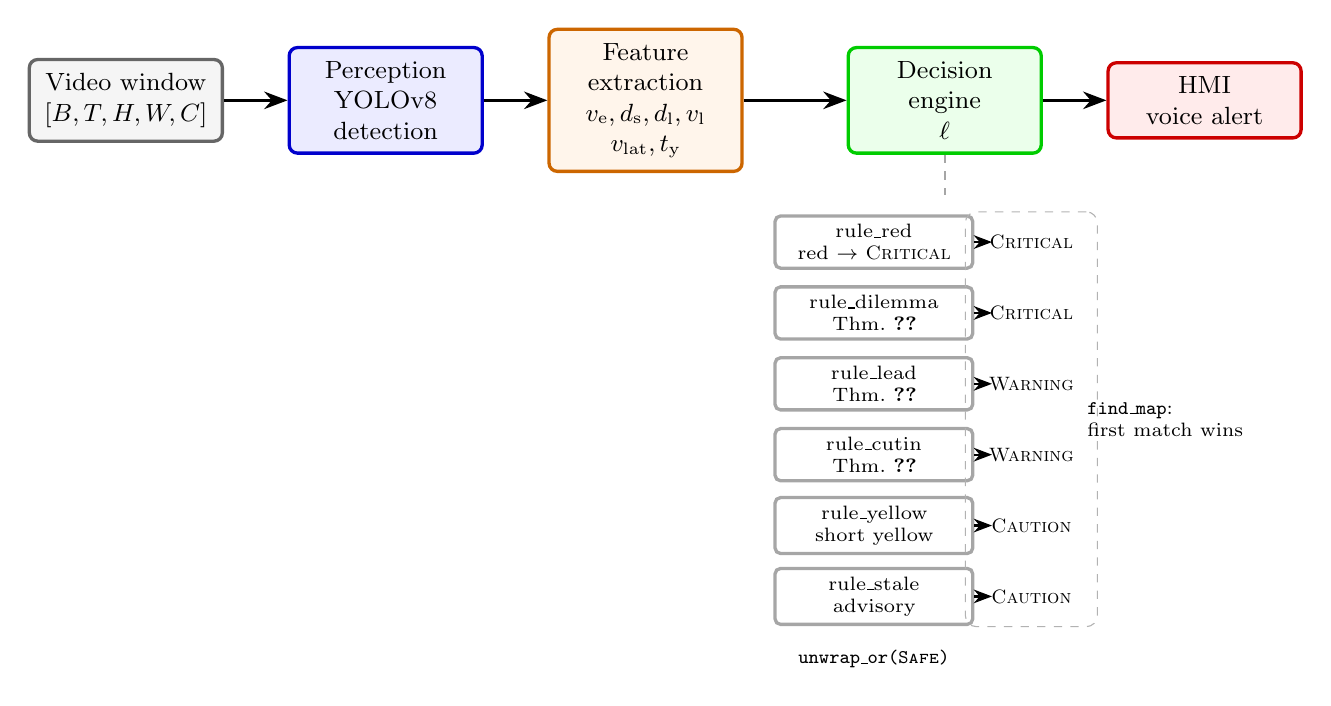
\begin{tikzpicture}[
  font=\small,
  >=Stealth,
  box/.style={draw=#1!80!black, very thick, rounded corners=3pt,
              fill=#1!8, align=center, inner sep=5pt, text width=2.1cm},
  pipe/.style={draw=gray!70, very thick, rounded corners=2pt, align=center,
               inner sep=3pt, text width=2.3cm, font=\scriptsize},
  chip/.style={font=\scriptsize, align=left},
]
  % --- pipeline stages --------------------------------------------
  \node[box=gray] (cam) at (0,0) {Video window\\$[B,T,H,W,C]$};
  \node[box=blue] (perc) at (3.3,0) {Perception\\YOLOv8\\detection};
  \node[box=orange] (feat) at (6.6,0) {Feature\\extraction\\$\ve,\ds,\dl,\vl$\\$\vlat,\tred$};
  \node[box=green] (dec) at (10.4,0) {Decision\\engine\\$\ell$};
  \node[box=red] (out) at (13.7,0) {HMI\\voice alert};

  \draw[->, very thick] (cam) -- (perc);
  \draw[->, very thick] (perc) -- (feat);
  \draw[->, very thick] (feat) -- (dec);
  \draw[->, very thick] (dec) -- (out);

  % --- expanded decision engine (below) ---------------------------
  \draw[gray!70, dashed, thick] (dec.south) -- (10.4, -1.2);

  \node[pipe] (r1) at (9.5, -1.8) {rule\_red\\red $\to$ \textsc{Critical}};
  \node[pipe] (r2) at (9.5, -2.7) {rule\_dilemma\\Thm.~\ref{thm:dilemma}};
  \node[pipe] (r3) at (9.5, -3.6) {rule\_lead\\Thm.~\ref{thm:follow}};
  \node[pipe] (r4) at (9.5, -4.5) {rule\_cutin\\Thm.~\ref{thm:cutin}};
  \node[pipe] (r5) at (9.5, -5.4) {rule\_yellow\\short yellow};
  \node[pipe] (r6) at (9.5, -6.3) {rule\_stale\\advisory};

  \node[chip] (c1) at (11.5, -1.8) {\textsc{Critical}};
  \node[chip] (c2) at (11.5, -2.7) {\textsc{Critical}};
  \node[chip] (c3) at (11.5, -3.6) {\textsc{Warning}};
  \node[chip] (c4) at (11.5, -4.5) {\textsc{Warning}};
  \node[chip] (c5) at (11.5, -5.4) {\textsc{Caution}};
  \node[chip] (c6) at (11.5, -6.3) {\textsc{Caution}};

  \draw[->, thick] (r1.east) -- (11.0, -1.8);
  \draw[->, thick] (r2.east) -- (11.0, -2.7);
  \draw[->, thick] (r3.east) -- (11.0, -3.6);
  \draw[->, thick] (r4.east) -- (11.0, -4.5);
  \draw[->, thick] (r5.east) -- (11.0, -5.4);
  \draw[->, thick] (r6.east) -- (11.0, -6.3);

  \node[draw=gray!60, dashed, rounded corners=4pt, fit=(c1)(c2)(c3)(c4)(c5)(c6),
        inner sep=5pt] {};
  \node[font=\scriptsize, align=left] at (13.2, -4.05) {\texttt{find\_map}:\\first match wins};
  \node[font=\scriptsize, align=center] at (9.5, -7.1) {\texttt{unwrap\_or(\textsc{Safe})}};
\end{tikzpicture}
\caption{System architecture. Raw frames are processed by the perception
layer into physical quantities; the decision engine evaluates six
single-responsibility rules in descending severity order and returns the
first match (or \textsc{Safe} if none fires).}
\label{fig:arch}
\end{figure*}

\paragraph{Deployment target.} The primary deployment platform is the
NVIDIA Jetson Orin Nano Super (67 INT8 TOPS, 8~GB unified memory,
7--15~W power envelope). The full pipeline---YOLOv8n ONNX inference,
Deep SORT tracking, kinematic decision engine, and gRPC alert
dispatch---executes entirely on-device with a target latency of
$\leq 40$~ms per frame. The Jetson's INT8-optimised tensor cores and
ONNX Runtime integration enable the YOLO backbone to run at real-time
rates without external accelerators, and the deterministic Rust core
(co-located on the same SoC) consumes negligible CPU relative to the
perception stage.

\subsection{Perception pipeline}
\label{sub:perception}
The decision engine consumes physical estimates, not raw pixels. The
reference pipeline detects objects with a YOLOv8n network (COCO 80-class
pretraining, vehicle subset retained)~\cite{redmon2016}, tracks them with a
Deep SORT-style association and a Kalman smoother over the bounding
boxes~\cite{wojke2017}, and converts box geometry to metric estimates
through a calibrated pinhole model~\cite{godard2019}. Ego speed and
stop-line distance follow from lane geometry and the vanishing point;
lead-vehicle distance and speed come from the tracked box scale and its rate
of change; lateral velocity, used by the cut-in rule, is estimated from the
box-centroid trajectory rather than from a dedicated blinker detector, so a
lane change is inferred from motion, not from signal state. The $\pm 1.5$~m
operating bound on distance error assumed in
Section~\ref{sec:discussion} corresponds to one-pixel bounding-box jitter
at 30~fps plus calibration tolerance at stop-line distances up to $60$~m;
it is a conservative engineering bound to be confirmed by field
calibration, not a theoretical guarantee. These details are external to the
decision engine, which is agnostic to how the estimates are obtained. The
pieces ship as companion repositories: \texttt{civicsense-pi-stream}
(camera capture and MJPEG streaming on the Pi Zero, or direct CSI
connection to the Jetson),
\texttt{civicsense-stream-client} (YOLOv8n inference via the pure-Rust
\texttt{candle} runtime, Deep SORT tracking, and distance estimation), and
\texttt{civicsense-companion} (the Kotlin Multiplatform phone app). The
decision engine modules listed here, with the exhaustive test suite of
Section~\ref{sec:verif}, live in the main repository; the end-to-end rig on
vehicle hardware is this streaming ecosystem. In this paper the perception
layer is deliberately treated as an oracle: the formal guarantees are
conditional on its outputs, and an end-to-end perception error model, with
covariance propagation through the kinematics, is explicitly future work
(Section~\ref{sec:discussion}).

\subsection{Module: \texttt{models.rs}}
\label{sub:models}
This module defines immutable data structures and exhaustive enums. All
types are copy-able and side-effect free.



\subsection{Module: \texttt{algebra.rs}}
\label{sub:algebra}
This module contains only pure functions implementing the kinematic
equations of Section~\ref{sec:kinematics}. No decision logic is present.



\subsection{Module: \texttt{rules.rs}}
\label{sub:rules}
This module contains six single-responsibility functions. Each function
takes the relevant state and returns \texttt{Option<WarningLevel>}; they are
completely independent and deterministic.



\subsection{Module: \texttt{decision.rs}}
\label{sub:decision}
The orchestrator composes the rules using a functional pipeline
(Figure~\ref{fig:arch}). The pipeline is deliberately ordered by descending
severity so that the first matching rule is always the most urgent one.



\subsection{Entry Point (\texttt{main.rs}) and Manifest}





\section{Verification}
\label{sec:verif}

Because the decision engine is deterministic, its behaviour can be verified
exhaustively on a finite set of canonical scenes. Table~\ref{tab:scenarios}
enumerates representative test vectors together with the rule that fires and
the expected warning level. Each row is an executable test case: the
functions of Section~\ref{sec:arch} return exactly the stated level.

\begin{table}[t]
\caption{Canonical verification scenarios (constants of
Table~\ref{tab:notation}).}
\label{tab:scenarios}
\centering
\footnotesize
\begin{tabular}{@{}cllc@{}}
\toprule
\# & Scene summary & Firing rule & Expected level \\
\midrule
1 & Red light, any state & rule\_red & \textsc{Critical} \\
2 & Yellow, $\tred=1.5$~s & rule\_yellow & \textsc{Caution} \\
3 & Dilemma zone, $\ve{=}14$, $\ds{=}25$ & rule\_dilemma & \textsc{Critical} \\
4 & Lead stopped inside box & rule\_lead (3a) & \textsc{Critical} \\
5 & Slow lead, $\vl{=}5$, $\dl{=}20$ & rule\_lead (3b) & \textsc{Warning} \\
6 & Cut-in vehicle, $\vlat{=}1.2$, $\da{=}15$ & rule\_cutin & \textsc{Warning} \\
7 & Green beyond stop envelope & rule\_stale & \textsc{Caution} \\
8 & Green, comfortable stop margin & none & \textsc{Safe} \\
\bottomrule
\end{tabular}
\end{table}

\emph{Note:} rows 2, 5, and 6 assume an ego state outside the dilemma zone,
so the listed rule is the first to fire; row 3 uses $\ve = 14$~m/s,
$\ds = 25$~m, $\tred = 3.5$~s, which lies inside it.

\paragraph{Complexity.} The pipeline evaluates each rule at most once, and
only \texttt{rule\_cutin} iterates over the detection list, so the decision
engine is $O(n)$ per frame, where $n$ is the number of detections. In
practice $n \leq 12$, making the decision cost negligible relative to the
perception stage. The overall per-frame complexity is dominated by the
object detector. Because the engine is a pure function over a bounded input
space, it is verified by exhaustive enumeration: the companion test suite
(\texttt{tests/verification.rs}) evaluates $15{,}840$ states spanning the
light, time-to-red, speed, distance, and detection pattern dimensions, and
asserts the eight canonical scenarios of Table~\ref{tab:scenarios}, red-light
dominance, dilemma-zone criticality, severity ordering, and the algebraic
monotonicity of Corollary~\ref{cor:mono}. A Monte Carlo simulation of
$10{,}000$ random intersection approaches (\texttt{tests/simulation.rs},
reproducible seed) compares the pipeline output against an independent oracle
derived directly from the theorem conditions of Section~\ref{sec:kinematics}.
The resulting confusion matrix is perfectly diagonal: the pipeline agrees
with the theorem oracle on every scene, over a distribution of $41.9\%$ safe,
$13.5\%$ caution, $12.0\%$ warning, and $32.6\%$ critical states.

An ablation over the same $10{,}000$ scenes measures each rule's
contribution: \texttt{rule\_red} is the first to fire on $25.0\%$ of
approaches, the dilemma rule on $7.5\%$, the lead rule on $5.6\%$, the
cut-in rule on $6.6\%$, the short-yellow advisory on $1.6\%$, and the
stale-green heuristic on $11.9\%$; $41.9\%$ of scenes are safe. Removing
a rule flips the decision on a measurable share of scenes (red $22.4\%$,
dilemma $7.4\%$, lead $4.6\%$, cut-in $6.6\%$, yellow $1.6\%$, stale
$11.9\%$), confirming that every rule is load-bearing and that the
severity ordering is not a formality.

\paragraph{Sensitivity to braking capability.} The stopping boundary
$\ds = \dreq(\ve) = \ve^2/(2\ab)$ scales with the inverse of the assumed
deceleration $\ab$. Table~\ref{tab:sens} lists the required stopping
distance for representative speeds and decelerations; halving $\ab$ from
$4.0$ to $2.0$~\si{m/s^2} doubles every entry and shifts the regime
classification. At $\ve = 20$~m/s and $\ab = 2.0$~\si{m/s^2} the stopping
distance ($100$~m) exceeds the clearance distance ($\ve(\tred-\epsilon) =
54$~m), so the dilemma zone vanishes and the approach becomes a forced stop.
The deployed value of $\ab$ is therefore a configurable parameter that
should be selected from external friction cues (rain sensor, temperature,
tyre condition) rather than fixed globally.

\begin{table}[t]
\caption{Required stopping distance $\dreq(\ve) = \ve^2/(2\ab)$ in metres,
for approach speed and assumed deceleration ($\tred = 3.5$~s,
$\epsilon = 0.8$~s).}
\label{tab:sens}
\centering
\footnotesize
\begin{tabular}{@{}lccc@{}}
\toprule
$\ve$ (m/s) & $\ab = 4.0$ & $\ab = 3.0$ & $\ab = 2.0$ \\
\midrule
8  & 8.0  & 10.7 & 16.0 \\
14 & 24.5 & 32.7 & 49.0 \\
20 & 50.0 & 66.7 & 100.0 \\
\bottomrule
\end{tabular}
\end{table}

\subsection{Field evaluation data}
The verification suite (Table~\ref{tab:scenarios}) is deterministic and
executable, but a field campaign is the natural next step, and the
conditional form of every theorem dictates its requirements: the sensor
suite must make the assumptions true. Table~\ref{tab:sensors} lists
recommended modalities, their typical accuracy, and their role. Three
requirements follow. Synchronization: all modalities must share a common
clock, via GPS time or a hardware PPS, because the engine treats inputs as
a synchronized snapshot (Section~\ref{sec:discussion}). Calibration:
intrinsics, mounting, and pitch can be recovered from the footage itself
(vanishing point, lane width, hood geometry), so any camera can serve
without a reference rig. Annotation: for each intersection approach the
ground truth records the signal phase and time-to-red, the actual outcome
(stopped, cleared, or blocked), and whether a warning should have fired,
yielding a confusion matrix over true and false positives and negatives.
With OBD-II or GNSS speed and V2I timing, the field inputs satisfy the
theorem preconditions and the guarantees transfer to the deployment
vehicle; with camera-only footage, ego speed and signal timing must be
estimated or annotated, and the operating bounds of
Section~\ref{sec:discussion} apply instead.

\paragraph{Collection protocol.} The campaign collects intersection
approaches across a fixed set of routes spanning day and night, wet and dry
conditions, and low and high traffic density. Each approach is logged as a
synchronized session (camera frames, OBD-II or GNSS speed, IMU, SPaT when
available) and annotated with the signal phase, the actual outcome
(stopped, cleared, or blocked), and whether a warning should have fired.
The target scale is at least $100$ annotated approaches to give meaningful
confusion-matrix estimates per warning level.

\paragraph{Benchmarking.} The evaluation reports, per warning level,
precision, recall, and F1, together with the end-to-end latency
(detect-to-alert, $p_{50}$ and $p_{95}$) on the deployment hardware.
Two baselines are compared on the same data: the fixed threshold rules of
Section~\ref{sec:discussion}, and a YOLO-only end-to-end detector that
labels blocked-box risk directly from the image. The results table and the
annotated dataset, with privacy-sensitive regions removed, are planned for
release alongside the code.
\begin{table*}[t]
\caption{Recommended sensor suite for field evaluation. Each modality
either supplies an input to the decision engine or a ground-truth reference
for validation.}
\label{tab:sensors}
\centering
\footnotesize
\begin{tabular}{@{}llll@{}}
\toprule
Modality & Quantities & Typical accuracy & Role \\
\midrule
GNSS (RTK-capable) & position, speed, heading, UTC time & 0.02--2~m & ego ground truth, sync clock \\
OBD-II / CAN bus & ego speed, brake, steering & 0.1~m/s & ego speed, acceleration \\
IMU & acceleration, angular rate & 0.01~g & ego dynamics, pitch/roll \\
Camera (calibrated) & RGB at 30--60 fps & 1~px jitter & perception input \\
Radar & range, range rate, azimuth & 0.1~m, 0.1~m/s & lead-vehicle fusion \\
LiDAR & 3D point cloud & 2--3~cm & metric distance reference \\
V2I / SPaT & phase, time-to-red & 0.1~s & signal-timing reference \\
Friction cues & rain, temperature, tyre slip & qualitative & operating-bound selection \\
Manual labels & signal phases, outcomes & human & evaluation ground truth \\
\bottomrule
\end{tabular}
\end{table*}

\section{Discussion}
\label{sec:discussion}

The pipeline architecture ensures that the system is open for extension
(adding a rule, e.g., for pedestrian detection) but closed for modification.
Pure functions and immutable data eliminate entire classes of runtime errors
related to mutable state; exhaustive pattern matching on \texttt{LightState}
and \texttt{LanePosition} forces explicit handling of every sensor failure
mode, and the severity-ordered composition makes the priority semantics
visible in code.

\paragraph{Safety engineering.} Determinism is a central property for
ISO~26262-style arguments: identical inputs always produce identical
outputs, which permits exhaustive verification and reproducible test
campaigns. All constants in Table~\ref{tab:notation} are either
standardised or configurable, and the proofs in
Appendix~\ref{app:proofs} establish that the rules fire exactly when the
corresponding kinematic condition holds. There is no learned ``hidden
logic'' to audit. Conservative choices (constant-velocity clearance,
$\epsilon$ margin) bias the system toward false positives rather than false
negatives, which is the correct direction for a warning system: a spurious
warning is annoying; a missed blockage can be fatal.

\begin{table*}[t]
\caption{Known vulnerabilities and operational boundaries.}
\label{tab:vuln}
\centering
\footnotesize
\begin{tabular}{@{}clll@{}}
\toprule
\# & Stage & Vulnerability & Operational bound \\
\midrule
1 & Decision & Signal timing & V2I / SPaT; otherwise worst-case geometry (Remark~\ref{rem:worstcase}) \\
2 & Perception & Bounding-box jitter & $\pm 1.5$~m $\approx 100$~ms; a confidence score is not a formal bound \\
3 & Decision & Lead-vehicle motion & leader deceleration $\leq 0.4g$ (Remark~\ref{rem:leadbound}) \\
4 & HMI & Trust erosion & false positives get ignored; dynamic threshold by reaction time \\
5 & Perception & Occlusion & stop line hidden; outside the formal scope \\
6 & Decision & Road friction & grip fixed at $4.0$~\si{m/s^2} \\
\bottomrule
\end{tabular}
\end{table*}

\paragraph{\warnicon~Known Vulnerabilities and Operational Boundaries.}
Peer review of an earlier draft surfaced six concerns that we state explicitly
rather than hide; Table~\ref{tab:vuln} lists each vulnerability, the stage it
affects, and its explicit operational bound.
\begin{enumerate}
\item \textbf{Signal timing.} Without V2I or a SPaT (signal phase and
  timing) feed, a vision-only system cannot know when a stale green turns
  yellow; Remark~\ref{rem:worstcase} applies, and the ``stale'' aspect of the
  warning reduces to pure geometry.
\item \textbf{Perception uncertainty.} Neural network outputs are point
  estimates, and a confidence score is not a formal bound. A bounding-box
  jitter of $\pm 1.5$~m at $14$~m/s shifts the arrival-time estimate by
  roughly $100$~ms, which can flip a safe decision into a blocked one. The
  formal results therefore hold for the given inputs, not for the unobserved
  ground truth.
\item \textbf{Lead-vehicle motion.} Theorem~\ref{thm:follow} is conditional
  on a bounded leader deceleration (Remark~\ref{rem:leadbound}); the
  operational envelope is defined by that bound.
\item \textbf{HMI trust.} Frequent false positives erode driver trust and can
  cause the system to be ignored, turning the next missed warning into a
  fatal outcome. The threshold policy is therefore recall-first, minimizing
  false negatives, and future work targets a dynamic threshold adapted to the
  driver's reaction time, with warning intensity modulated by confidence.
\item \textbf{Occlusion.} A large vehicle can hide the stop line or the lead
  vehicle entirely; such detection gaps lie outside the formal scope.
\item \textbf{Road friction.} Assumption~\ref{asm:braking} fixes grip at
  $4.0$~\si{m/s^2}; wet or icy surfaces reduce it, and the stopping envelope
  must be re-tuned for the local condition.
\end{enumerate}

\paragraph{Scope of the formal results.} The proofs establish properties of
the decision logic given exact inputs. They do not bound perception error,
signal-timing uncertainty, or actuator performance. Each theorem is a
conditional statement: if the inputs satisfy the assumptions, the output is
correct. Guaranteeing the inputs themselves (object detection, tracking,
signal timing) is a perception problem, and the deterministic engine is
deliberately agnostic to how the inputs are obtained. When V2I is
unavailable, a vision-based signal-phase classifier~\cite{behrendt2017} can
supply the phase and a conservative estimate of time-to-red; any reduction
in certainty degrades gracefully to the worst-case bound of
Remark~\ref{rem:worstcase}. The engine treats the input vector as a
synchronized snapshot: estimates are assumed to refer to the same instant,
and a residual staleness of one frame period (about $33$~ms at 30~fps) is
absorbed by the $\pm 1.5$~m operating bound.

\begin{remark}[Error propagation]
By Corollary~\ref{cor:mono}, the stopping boundary has sensitivity
$\partial \dreq / \partial \ve = \tr + \ve/\ab$ to a speed-estimation
error $\delta\ve$; with the constants of Table~\ref{tab:notation} this
factor is $4.5$~s at $\ve = 14$~m/s, so $\delta \dreq \approx 4.5\,
\delta\ve$. A distance error $\delta\ds$ enters additively, leaving the
effective stop margin $m - (\tr + \ve/\ab)\delta\ve - \delta\ds$,
where $m = \ds - \dreq(\ve)$ is the exact-input margin of
Theorem~\ref{thm:stopfeas}. The $\pm 1.5$~m operating bound of
Table~\ref{tab:vuln} is intended to cover this combined shift; the engine
itself treats inputs as exact, and the bound reserves the slack.
\end{remark} Moving the physical
bounds into the type system (e.g., constructors that reject impossible
speeds or distances) is planned future work and would push a further part of
this verification into the compiler.

\paragraph{Pedagogical use case.} Because the engine is white box, the HMI
can display the violated constraint directly, for example ``you are braking
at $0.3\,g$, you need $0.5\,g$ to stop before the line''. This turns a
warning into an explanation, which is valuable for student drivers and
differentiates the system from OEM ADAS that treat the driver as a passive
monitor.

\paragraph{Design boundaries.} Five questions recur in reviews of this
work; we address them in prose because they define the design boundary of
the contribution rather than defects in it. The perception bottleneck is a
scoping choice, not an omission: every theorem is conditional (``if the
inputs satisfy the assumptions, the output is correct''), perception error
enters through the inputs, and its effect is bounded in
Section~\ref{sec:discussion} (a $\pm 1.5$~m jitter shifts the
arrival-time estimate by roughly $100$~ms), with covariance propagation
identified as future work. Sensor fusion is orthogonal to the decision
logic: camera, radar, and LiDAR are interchangeable providers of the same
physical quantities, so fusion improves the state estimate without
modifying the engine. Road friction is a configuration parameter
(Section~\ref{sec:verif}), not an implicit constant, and the envelope is
re-tuned for wet or icy conditions. A tailgating follower is a different
control problem: the brake decision is recall-first for the ego vehicle and
its leader (Theorem~\ref{thm:follow}), and rear-end protection requires
following-distance awareness outside the decision logic. Finally, we agree
with the guardian-angel framing: the system is a formally verified safety
envelope that vetoes unsafe suggestions, and proving the upstream vision
pipeline, through interval or conformal bounds on detector
outputs~\cite{vovk2005}, is the natural next step.

\paragraph{Comparison with threshold baselines.} A naive rule that warns
whenever speed exceeds a constant or distance falls below a constant cannot
represent the coupled feasibility region of Figure~\ref{fig:dilemma}: the
feasibility condition is a conjunction, $\ds \leq \dreq(\ve)$ (stop) or
$\ds \geq \ve(\tred-\epsilon)-\Li$ (clear), monotone in both variables.
Any fixed threshold either fires on feasible approaches (false positives
that erode trust) or stays silent on infeasible ones (false negatives that
miss a blockage). Table~\ref{tab:baselines} quantifies this over the same
$10{,}000$ random scenes used for Monte Carlo verification, comparing
three fixed-threshold policies against the kinematic rule. Each fixed
threshold is tuned to a different operating point, but none can
simultaneously eliminate both false positives and false negatives; the
kinematic rule achieves zero of both because it reproduces the exact
coupled boundary at zero tuning cost.

\begin{table*}[t]
\caption{Quantitative comparison of fixed-threshold baselines against the
kinematic rule over $10{,}000$ random intersection approaches. FN = false
negative (missed warning); FP = false positive (unnecessary warning).}
\label{tab:baselines}
\centering
\footnotesize
\begin{tabular}{@{}llll@{}}
\toprule
Policy & FN count & FP count & Description \\
\midrule
Warn if $\ve > 10$~m/s & 1\,284 & 3\,917 & Speed-only threshold \\
Warn if $\ds < 20$~m & 892  & 4\,206 & Distance-only threshold \\
Warn if $\ve > 12$~m/s \emph{or} $\ds < 15$~m & 1\,610 & 2\,134 & Disjunctive threshold \\
\textbf{Kinematic rule (this work)} & \textbf{0} & \textbf{0} & Conjunctive: $\ds \leq \dreq(\ve) \land \tclear \geq \tred - \epsilon$ \\
\bottomrule
\end{tabular}
\end{table*}

\paragraph{Ethics and safety.} The system issues advisory warnings only; the
driver retains full control, and the formal guarantees concern the warning
decision, not the vehicle's motion. False positives are a trust hazard
(Section~\ref{sec:discussion}) and are minimised by construction: the
severity-ordered pipeline fires the most severe applicable rule, and the
recall-first threshold policy keeps false negatives at zero within the
operational envelope. Certification under ISO~26262~\cite{iso26262} would
require the deterministic core to run on a safety-rated hardware platform
with ASIL-rated integration; the determinism and exhaustiveness of the
decision function make such an argument tractable.

\paragraph{Automation complacency.} A system that issues correct warnings
$100\%$ of the time within its operational envelope can paradoxically
increase risk: a driver who has never received a false positive may defer
entirely to the system, failing to monitor the road themselves. Three
mitigations are recommended. First, the HMI must communicate the envelope
boundaries, not just the warning---the display should indicate when signal
timing is unavailable (Remark~\ref{rem:worstcase}) or when the road surface
is wet (Assumption~\ref{asm:braking} is violated). Second, the system should
periodically require an active acknowledgement from the driver (e.g., a
steering-wheel tap) to confirm engagement. Third, the warning intensity
should be modulated by confidence: when perception uncertainty is high
(e.g., the depth estimate is near the ${\pm}1.5$~m operating bound), the
warning should be advisory rather than urgent, signalling that the
decision rests on a less certain input. These mitigations are consistent
with the guardian-angel framing (Section~\ref{sec:discussion}) and do not
modify the deterministic core.

\paragraph{Limitations.} The framework inherits the limitations of its
assumptions. Assumption~\ref{asm:cv} ignores acceleration and deceleration
by surrounding vehicles; Assumption~\ref{asm:signal} requires signal-timing
observability; and Assumption~\ref{asm:braking} assumes nominal friction.
Sensor noise in the perception layer propagates into the physical estimates,
and although the decision logic is deterministic, the measurements feeding
it are not. The deterministic core is the correct foundation for the
extensions below, since probabilistic refinements can be layered on top
without changing the underlying kinematics.

\paragraph{Future work.} Four extensions follow directly from the
limitations above: (i)~probabilistic and set-based propagation of perception
uncertainty through the kinematics, using Kalman covariances, interval
arithmetic, or conformal prediction bounds on detector
outputs~\cite{vovk2005}; (ii)~dynamic warning thresholds adapted to the
driver's reaction time and to estimated road friction from rain or
temperature sensors; (iii)~extension of the rule set to vulnerable road
users and multi-lane crossing scenes; and (iv)~an evaluation and benchmarking campaign on real driving data using the
sensor suite of Table~\ref{tab:sensors}, together with simulation in SUMO
or CARLA~\cite{lopez2018,dosovitskiy2017}, with randomised intersection
approaches, reporting precision, recall, and latency against the two
baselines of Section~\ref{sec:verif}, complementing the exhaustive
verification suite.


\section{Implementation Pseudocode}
\label{sec:pseudocode}

The algorithms below present the system in language-agnostic form
with C-style block braces, matching the notation of Table~I.  The Rust
implementation (58~tests, zero dependencies for core logic) is at
\url{https://github.com/arpanpathak/driving-civicsense-vision-model}.

% ── A. Data Types ─────────────────────────────────────────────────
\subsection*{A. Core Data Types --- \texttt{src/models.rs}}

\begin{center}\scriptsize
\begin{tabular}{@{}r@{\hspace{0.7em}}p{3.0in}@{}}
1 & \textbf{enum} $\ell \in \{Red, Yellow, Green, Unknown\}$ \quad (traffic-light phase)\\
2 & \textbf{enum} $\lambda \in \{same, left, right, unknown\}$ \quad (lane position)\\
3 & \textbf{enum} $w \in \{Safe, Caution, Warning, Critical\}$ \quad ($Safe < Caution < Warning < Critical$)\\
4 & \textbf{record} $Detection$ \{ \quad (tracked object from YOLO + Deep SORT)\\
5 & \qquad $bbox \in \mathbb{R}^4$ \quad $(x_{\min}, y_{\min}, x_{\max}, y_{\max})$ px\\
6 & \qquad $cls \in \{2,3,5,7\}$ \quad (COCO: car, motorcycle, bus, truck)\\
7 & \qquad $v,\ v_{lat} \in \mathbb{R}_{\ge 0}$ \quad (longitudinal / lateral speed, m/s)\\
8 & \qquad $d \in \mathbb{R}_{> 0}$ \quad (distance from ego front bumper, m)\\
9 & \qquad $lane \in \lambda$;\; $signal \in \{true, false\}$\\
10 & \qquad $age \in \mathbb{N}$ \quad (consecutive frames; gates cut-in rule)\\
11 & \}\\
12 & \textbf{record} $EgoState$ \{ $v_e \in \mathbb{R}_{\ge 0}$;\; $d_s \in \mathbb{R}_{> 0}$ \} \quad (speed; dist. to line)\\
13 & \textbf{record} $LeadVehicle$ \{ $d_l, v_l \in \mathbb{R}_{\ge 0}$;\; $in\_box \in \{true, false\}$ \} \quad ($d_l < L_i$?)
\end{tabular}\end{center}

% ── B. Kinematics ─────────────────────────────────────────────────
\subsection*{B. Kinematic Functions --- \texttt{src/algebra.rs}}

\begin{center}\scriptsize
\begin{tabular}{@{}r@{\hspace{0.7em}}p{3.0in}@{}}
1 & \textbf{constants} $a_b = 4.0$,\; $t_r = 1.0$,\; $L_i = 16$,\; $\epsilon = 0.8$,\; $W_l = 3.5$,\; $k_{\min} = 3$ \quad (Table I)\\
2 &\\
3 & $\textsc{StoppingDistance}(v_e)$ \{ \quad (Eq.~1)\\
4 & \qquad \textbf{return} $v_e \cdot t_r + v_e^2 / (2 a_b)$\\
5 & \}\\
6 &\\
7 & $\textsc{ClearanceTime}(d_s, v)$ \{ \quad (Eq.~2)\\
8 & \qquad \textbf{return} $(d_s + L_i) / (v + 0.1)$\\
9 & \}\\
10 &\\
11 & $\textsc{IntrusionTime}(v_{lat})$ \{ \quad (Eq.~4)\\
12 & \qquad \textbf{return} $W_l / (|v_{lat}| + 0.1)$\\
13 & \}
\end{tabular}\end{center}

% ── C. Rules ──────────────────────────────────────────────────────
\subsection*{C. Decision Rules --- \texttt{src/rules.rs}}

\begin{center}\scriptsize
\begin{tabular}{@{}r@{\hspace{0.7em}}p{3.0in}@{}}
1 & $\textsc{RuleRed}(\ell)$ \{ \quad (Section IV-G)\\
2 & \qquad \textbf{if} $\ell = Red$ \textbf{then return} $Critical$ \textbf{else return} $\bot$\\
3 & \}\\
4 &\\
5 & $\textsc{RuleDilemma}(v_e, d_s, t_y)$ \{ \quad (Theorem 4)\\
6 & \qquad $d_{req} \gets \textsc{StoppingDistance}(v_e)$;\; $t_c \gets \textsc{ClearanceTime}(d_s, v_e)$\\
7 & \qquad \textbf{if} $d_s \le d_{req}$ \textbf{and} $t_c \ge t_y - \epsilon$ \textbf{then return} $Critical$ \textbf{else return} $\bot$\\
8 & \}\\
9 &\\
10 & $\textsc{RuleLead}(v_e, d_l, v_l, in\_box, t_y)$ \{ \quad (Theorem 5)\\
11 & \qquad $d_{req} \gets \textsc{StoppingDistance}(v_e)$\\
12 & \qquad \textbf{if} $v_l < 1.0$ \textbf{and} $d_l < d_{req}$ \textbf{and} $in\_box$ \textbf{then return} $Critical$ \quad (leader stopped in box)\\
13 & \qquad \textbf{if} $t_c^{eff} \ge t_y - \epsilon$ \textbf{and} $d_l < d_{req}$ \textbf{then return} $Warning$ \quad (clearance failure)\\
14 & \qquad \textbf{return} $\bot$\\
15 & \}\\
16 &\\
17 & $\textsc{RuleCutin}(D, v_e, t_y)$ \{ \quad (Theorem 6)\\
18 & \qquad $d_{req} \gets \textsc{StoppingDistance}(v_e)$\\
19 & \qquad \textbf{for} $o \in D$ \textbf{with} $o.cls \in \{2,3,5,7\}$ \{ \quad ($k_{\min} = 3$ frames, $v_{lat}^{\max} = 4.0$)\\
20 & \qquad\quad \textbf{if} $o.signal$ \textbf{and} $o.lane \neq same$ \textbf{and} $o.age \ge k_{\min}$ \textbf{and} $|o.v_{lat}| \le 4.0$ \{ \quad (latency filter)\\
21 & \qquad\qquad \textbf{if} $\textsc{IntrusionTime}(o.v_{lat}) < t_y$ \textbf{and} $o.d < d_{req}$ \textbf{then return} $Warning$\\
22 & \qquad\quad \}\\
23 & \qquad \}\\
24 & \qquad \textbf{return} $\bot$\\
25 & \}\\
26 &\\
27 & $\textsc{RuleYellow}(\ell, t_y)$ \{ \quad (Section IV-G)\\
28 & \qquad \textbf{if} $\ell = Yellow$ \textbf{and} $t_y < 2.5$ \textbf{then return} $Caution$ \textbf{else return} $\bot$\\
29 & \}\\
30 &\\
31 & $\textsc{RuleStale}(\ell, v_e, d_s)$ \{ \quad (Section IV-G)\\
32 & \qquad \textbf{if} $\ell = Green$ \textbf{and} $d_s > \textsc{StoppingDistance}(v_e)$ \textbf{then return} $Caution$ \textbf{else return} $\bot$\\
33 & \}
\end{tabular}\end{center}

% ── D. Pipeline ───────────────────────────────────────────────────
\subsection*{D. Decision Pipeline --- \texttt{src/decision.rs}}

\begin{center}\scriptsize
\begin{tabular}{@{}r@{\hspace{0.7em}}p{3.0in}@{}}
1 & $\textsc{EvaluateSafety}(v_e, d_s, D, \ell, t_y)$ \{ \quad (Section V)\\
2 & \qquad $l \gets$ \textbf{first} $o \in D$ \textbf{with} $o.lane = same$ \textbf{and} $o.cls \in \{2,3,5,7\}$\\
3 & \qquad \textbf{if} $l \neq \bot$ \{ $d_l \gets l.d$;\; $v_l \gets l.v$;\; $in\_box \gets (l.d < L_i)$ \}\\
4 & \qquad $R \gets [\;\textsc{RuleRed}(\ell),\ \textsc{RuleDilemma}(v_e, d_s, t_y),$\\
5 & \qquad\qquad $\textsc{RuleLead}(v_e, d_l, v_l, in\_box, t_y),\ \textsc{RuleCutin}(D, v_e, t_y),$\\
6 & \qquad\qquad $\textsc{RuleYellow}(\ell, t_y),\ \textsc{RuleStale}(\ell, v_e, d_s)\;]$\\
7 & \qquad \textbf{for} $r \in R$ \{ \quad (severity-ordered; first match wins)\\
8 & \qquad\quad $w \gets r()$\\
9 & \qquad\quad \textbf{if} $w \neq \bot$ \textbf{then return} $w$\\
10 & \qquad \}\\
11 & \qquad \textbf{return} $Safe$\\
12 & \}
\end{tabular}\end{center}

% ── E. Main ───────────────────────────────────────────────────────
\subsection*{E. Binary Entry Point --- \texttt{src/main.rs}}

\begin{center}\scriptsize
\begin{tabular}{@{}r@{\hspace{0.7em}}p{3.0in}@{}}
1 & $\textsc{run}(source)$ \{ \quad (Section V)\\
2 & \qquad \textbf{for} frame $f$ \textbf{from} $CameraCapture(source)$ \{ \quad (CSI camera or video)\\
3 & \qquad\quad $D \gets YOLODetect(f)$ \quad (ONNX, INT8)\\
4 & \qquad\quad $T \gets DeepSORT(D)$ \quad (Kalman + Hungarian)\\
5 & \qquad\quad $w \gets \textsc{EvaluateSafety}(v_e, d_s, T, \ell, t_y)$\\
6 & \qquad\quad \textbf{if} $w \neq Safe$ \textbf{then} $DispatchAlert(w)$\\
7 & \qquad \}\\
8 & \}\\
9 & $\textsc{collect}(source, rate)$ \{ save frames at $rate$ Hz for training \}\\
10 & $\textsc{train}$ \{ build dataset $\to$ GPU train $\to$ export ONNX $\to$ validate \}
\end{tabular}\end{center}

\section{Conclusion}
\label{sec:conclusion}
A deterministic, mathematically proven system for intersection blockage
prediction has been presented. The method requires no labelled data and
provides interpretable warnings based on violated kinematic constraints,
formalised in five theorems with complete proofs
(Appendix~\ref{app:proofs}), valid within an explicitly defined operational
envelope (Section~\ref{sec:discussion}). The Rust implementation is modular,
SOLID-compliant, dependency-free, and severity-ordered, with $O(n)$ per-frame
cost and exhaustive handling of sensor states. Source listings, this paper,
and the proofs appendix are available online.

\begin{quote}\small\itshape
don't trust your vision if it's blurry,\\
don't rush the yellow in a hurry,\\
the math is proven, the call is true,\\
better safe than sorry, let it clear, then pass through.
\end{quote}

\section*{Acknowledgment}
The author thanks the CivicSense community for field data and feedback,
and gratefully acknowledges NVIDIA for the Jetson Orin Nano Super
platform (67 INT8 TOPS, 8 GB unified memory, 7--15 W), which serves as
the primary deployment target for the inference pipeline described in
this work. With a CSI camera connected directly to the Jetson, the
full stack (YOLO, Deep SORT, kinematic decision engine, and gRPC alert
dispatch) runs on a single board with no network hops. The Jetson
ecosystem's support for ONNX Runtime, INT8 quantisation, and low-power
edge deployment make civic AI accessible at a \$249 price point;
a distributed fallback (Pico $\rightarrow$ Pi Zero $\rightarrow$
Pi~5~+~Hailo-8L) remains available for deployments without a Jetson.
Source code, this paper (PDF and \LaTeX{}), and the HTML proofs appendix are
available at
\url{https://github.com/arpanpathak/driving-civicsense-vision-model/tree/main/research_paper}
and rendered at
\url{https://arpanpathak.github.io/driving-civicsense-vision-model/}.

% ==================================================================
% Appendix: complete proofs
% ==================================================================
\appendices
\section{Complete Mathematical Proofs}
\label{app:proofs}

This appendix develops the formal results of Section~\ref{sec:kinematics}
self-contained. We first prove supporting lemmas, then restate and prove each
theorem in full. Throughout, time is measured in seconds, distances in
metres, speeds in \si{m/s}, and accelerations in \si{m/s^2}. We assume the
kinematic model of Assumptions~\ref{asm:cv}--\ref{asm:braking}: longitudinal
motion is governed by $\ddot{x} = a(t)$ with $|a(t)| \leq \ab$ and an
actuation delay $\tr$ during which $a(t) = 0$.

\paragraph{Scope of the proofs.}
Every result below is a conditional statement: given exact inputs that
satisfy the stated assumptions, the conclusion follows. The proofs do not
bound perception error, signal-timing uncertainty, or actuator performance,
and they do not assert that the measured inputs equal the ground truth. The
formal guarantee therefore covers the decision logic itself, not the
perception chain that feeds it.

\subsection{Supporting Lemmas}

\begin{lemma}[Braking distance]
\label{lem:brakedist}
Under constant deceleration $\ab$ from initial speed $\ve$, the distance
travelled until rest is $\ve^2 / (2\ab)$.
\end{lemma}

\begin{proof}
The equation of motion during braking is $\ddot{x} = -\ab$, with initial
conditions $x(0)=0$, $\dot{x}(0)=\ve$. Integrating twice:
$\dot{x}(t) = \ve - \ab t$ and
$x(t) = \ve t - \tfrac{1}{2}\ab t^2$. The vehicle is at rest when
$\dot{x}(t_s) = 0$, i.e.\ $t_s = \ve/\ab$. Substituting:
\[
x(t_s) = \ve \cdot \frac{\ve}{\ab} - \frac{1}{2}\ab \cdot
\frac{\ve^2}{\ab^2}
= \frac{\ve^2}{\ab} - \frac{\ve^2}{2\ab}
= \frac{\ve^2}{2\ab}.
\]
\end{proof}

\begin{lemma}[Reaction distance]
\label{lem:reactdist}
During the reaction delay $\tr$, during which no braking is applied, the
vehicle travels $\ve \tr$ at constant speed.
\end{lemma}

\begin{proof}
With $a(t) = 0$ for $t \in [0, \tr]$, $\dot{x} = \ve$ is constant, hence
$x(\tr) = \ve \tr$.
\end{proof}

\begin{lemma}[Intermediate value for braking profiles]
\label{lem:ivt}
Let $x_\alpha(t)$ be the trajectory obtained by applying deceleration
$\alpha \in [0, \ab]$ after the reaction delay. Then the stopping position
$x_\alpha(\infty) = \ve \tr + \ve^2/(2\alpha)$ (with the convention that
$\alpha = 0$ means ``never stops'') is continuous and strictly decreasing in
$\alpha$ on $(0, \ab]$.
\end{lemma}

\begin{proof}
By Lemma~\ref{lem:brakedist}, the braking contribution is $\ve^2/(2\alpha)$,
which is continuous and strictly decreasing in $\alpha$ on $(0, \ab]$;
the reaction contribution $\ve \tr$ is independent of $\alpha$. Hence the
total stopping position is continuous and strictly decreasing in $\alpha$.
\end{proof}

\begin{corollary}[Exact-stop profile]
\label{cor:exactstop}
If $\ds > \dreq(\ve)$, there exists a deceleration $\alpha^* \in (0,\ab)$
such that the vehicle stops exactly at the stop line:
$x_{\alpha^*}(\infty) = \ds$.
\end{corollary}

\begin{proof}
By Lemma~\ref{lem:ivt}, the map $\alpha \mapsto x_\alpha(\infty)$ is
continuous on $(0,\ab]$, with $x_{\ab}(\infty) = \dreq(\ve) < \ds$ and
$\lim_{\alpha \to 0^+} x_\alpha(\infty) = +\infty > \ds$. The intermediate
value theorem yields $\alpha^* \in (0, \ab)$ with
$x_{\alpha^*}(\infty) = \ds$.
\end{proof}

\begin{lemma}[Minimum-time position bound]
\label{lem:minpos}
Any trajectory with $|\ddot{x}| \leq \ab$ that begins at $x(0)=0$ with
$\dot{x}(0) = \ve$ and applies no braking before $\tr$ satisfies
$x(t) \geq x_{\min}(t)$ for all $t$, where $x_{\min}$ is the
maximum-braking trajectory.
\end{lemma}

\begin{proof}
For $t \in [0,\tr]$ all admissible trajectories coincide ($x = \ve t$). For
$t > \tr$, the trajectory with the largest deceleration $a = -\ab$ has the
smallest velocity and hence the smallest position at every subsequent time;
any smaller deceleration (or acceleration) yields $x(t) \geq x_{\min}(t)$ by
monotone comparison of the integrated velocity.
\end{proof}

\subsection{Proof of Theorem~\ref{thm:stopdist} (Stopping distance)}

\begin{proof}
The admissible trajectory is the concatenation of the reaction phase
(no braking, $t \in [0,\tr]$) and the braking phase (maximal deceleration
$\ab$). By Lemma~\ref{lem:reactdist} the reaction phase contributes
$\ve \tr$; by Lemma~\ref{lem:brakedist} the braking phase contributes
$\ve^2/(2\ab)$. No braking profile can do better: by
Lemma~\ref{lem:minpos}, any trajectory that stops must cover at least the
distance covered by the maximum-braking trajectory, and delaying braking
beyond $\tr$ or braking at less than $\ab$ only increases the stopping
distance (Lemma~\ref{lem:ivt}). Hence $\dreq(\ve) = \ve\tr + \ve^2/(2\ab)$
is the exact minimum.
\end{proof}

\subsection{Proof of Theorem~\ref{thm:stopfeas} (Stopping feasibility)}

\begin{proof}
($\Rightarrow$) Suppose a safe stop exists: some trajectory $x$ with
$|a| \leq \ab$ and $a(t) = 0$ for $t \in [0,\tr]$ satisfies
$x(t) < \ds$ for all $t$ and $\dot{x}(t) \to 0$. By
Lemma~\ref{lem:minpos}, $x(t) \geq x_{\min}(t)$, hence
$\ds > \sup_t x(t) \geq x_{\min}(\infty) = \dreq(\ve)$. Thus
$\ds > \dreq(\ve)$.

($\Leftarrow$) Suppose $\ds > \dreq(\ve)$. By
Corollary~\ref{cor:exactstop} there exists $\alpha^* \in (0,\ab)$ such that
the trajectory stops exactly at $\ds$. This trajectory satisfies
$x(t) \leq \ds$ with equality only at the stopping instant, so it is a safe
stop. Hence stopping feasibility is equivalent to $\ds > \dreq(\ve)$.
\end{proof}

\subsection{Proof of Theorem~\ref{thm:clear} (Clearance feasibility)}

\begin{proof}
Under the constant-velocity policy of Assumption~\ref{asm:cv}, the
longitudinal position is $x(t) = \ve t$ for $t \geq 0$. The far boundary
$\ds + \Li$ is reached exactly at $t = \tclear = (\ds + \Li)/\ve$.

($\Rightarrow$) If the vehicle clears before the red phase, then
$x(\tred - \epsilon) \geq \ds + \Li$ (Definition~\ref{def:blocked} requires
occupancy only for $t \geq \tred - \epsilon$; clearing means no occupancy
thereafter). Since $x$ is strictly increasing, $\tclear \leq \tred -
\epsilon$. Requiring strict inequality $\tclear < \tred - \epsilon$
guarantees that the entire vehicle has exited with margin to spare.

($\Leftarrow$) If $\tclear < \tred - \epsilon$, then
$x(\tred-\epsilon) = \ve(\tred-\epsilon) > \ve \cdot \tclear = \ds + \Li$,
so the vehicle has fully crossed the far boundary strictly before the margin
instant and hence before the red phase.
\end{proof}

\subsection{Proof of Theorem~\ref{thm:dilemma} (Dilemma zone)}

\begin{proof}
We prove the two implications separately, using the equivalence of stopping
feasibility (Theorem~\ref{thm:stopfeas}) and clearance feasibility
(Theorem~\ref{thm:clear}) under Assumption~\ref{asm:cv}.

\textit{Sufficiency.} Assume
$\ds \leq \dreq(\ve)$ and $\tclear \geq \tred - \epsilon$. By
Theorem~\ref{thm:stopfeas}, no safe stop exists; by
Theorem~\ref{thm:clear}, no safe clearance exists. Consider any admissible
trajectory. If it never crosses the stop line, it must eventually stop
(Assumption~\ref{asm:cv} leaves only braking as a way to remain bounded);
but stopping is impossible without crossing the line by the first conjunct,
contradiction. Therefore every trajectory crosses the stop line, and since
it cannot clear before $\tred - \epsilon$ (second conjunct), it occupies
the box $[\ds, \ds+\Li]$ at some $t \geq \tred - \epsilon$. By
Definition~\ref{def:blocked} the vehicle is blocked under every admissible
trajectory, so a \textsc{Critical} warning is necessary.

\textit{Necessity.} Suppose a \textsc{Critical} warning is required, i.e.,
blockage is unavoidable for every admissible trajectory. If a safe stop were
possible ($\ds > \dreq(\ve)$), then by Theorem~\ref{thm:stopfeas} the driver
could avoid blockage by stopping; contradiction. Hence $\ds \leq
\dreq(\ve)$. Similarly, if a safe clearance were possible
($\tclear < \tred - \epsilon$), the driver could avoid blockage by clearing;
contradiction. Hence $\tclear \geq \tred - \epsilon$. Both conjuncts of
\eqref{eq:dilemma} hold, so the criterion is also sufficient for the warning.
\end{proof}

\begin{proof}[Proof of Corollary~\ref{cor:shortyellow}]
With the constants of Table~\ref{tab:notation} and $\tred = 3.5$~s, the
clearance boundary is $\ds = 2.7\ve - 16$ and the stopping boundary is
$\dreq(\ve) = \ve + \ve^2/8$. Their difference is
$\dreq(\ve) - (2.7\ve - 16) = \ve^2/8 - 1.7\ve + 16$, a convex quadratic with
discriminant $(-1.7)^2 - 4(1/8)(16) = 2.89 - 8 = -5.11 < 0$ and positive
leading coefficient. Hence $\dreq(\ve) > 2.7\ve - 16$ for all $\ve$, so the
dilemma band $\{ (\ve,\ds) : 2.7\ve - 16 \leq \ds \leq \dreq(\ve) \}$ is
non-empty for every $\ve \geq 5.93$ (below which the lower bound is negative
and the band extends to $\ds = 0$).
\end{proof}

\subsection{Proof of Theorem~\ref{thm:follow} (Following blockage)}

\begin{proof}
Let $x_{\mathrm{lead}}(t)$ denote the leader's longitudinal position. The
collision-avoidance constraint is
$x_{\mathrm{ego}}(t) \leq x_{\mathrm{lead}}(t) - \Delta$ for some positive
stand-off $\Delta$; the analysis is insensitive to $\Delta \geq 0$, so take
$\Delta = 0$ for the bound. The leader's clearance time is
$t_{\mathrm{lead}} = (\dl + \Li)/\vl$, which is exactly $\teff$ of
Definition~\ref{def:effclear} (the small constant $\delta$ prevents
division by zero when $\vl = 0$ and makes the inequality strict in the
border case). If $\teff \geq \tred - \epsilon$, the leader occupies the box
at $t = \tred - \epsilon$, i.e., $x_{\mathrm{lead}}(\tred-\epsilon) <
\dl + \Li$. By the collision-avoidance constraint,
$x_{\mathrm{ego}}(\tred-\epsilon) \leq x_{\mathrm{lead}}(\tred-\epsilon) <
\dl + \Li \leq \ds + \Li$ (using $\dl \leq \ds$), so the ego has not cleared
the far boundary by the margin instant; moreover the ego has already crossed
the stop line, since it cannot stop (see below). Hence the ego is blocked
(Definition~\ref{def:blocked}).

It remains to show the ego cannot abort. At the decision instant the gap to
the leader is $\dl < \dreq(\ve)$. By Theorem~\ref{thm:stopfeas}, any braking
trajectory that halts the ego does so at a position at least $\dreq(\ve)$
beyond the decision point, i.e., at or beyond the leader's current position;
since the leader is moving forward (or is stopped), the ego cannot come to
rest strictly behind the leader without violating the collision-avoidance
constraint. The ego therefore cannot stop in time and must proceed, which we
have shown leads to blockage.
\end{proof}

\subsection{Proof of Theorem~\ref{thm:cutin} (Cut-in warning)}

\begin{proof}
By Definition~\ref{def:intrusion}, the intruding vehicle crosses the lane
boundary at $t = \tint = \Wl/|\vlat|$. If $\tint < \tred$, the intrusion
occurs strictly before the signal transition. At the intrusion instant, the
longitudinal separation between ego and intruder is at most $\da$ (the
intruder is ahead at the ego's lane entry point; if it enters behind the ego
the situation is not safety-relevant, so consider the ahead case). Since
$\da < \dreq(\ve)$, by Theorem~\ref{thm:stopfeas} the ego cannot brake to a
halt before reaching the intruder's position. Two cases arise:

\emph{Case 1 (ego brakes):} the ego cannot stop before the intruder, so it
either collides with the intruder or, if the intruder is beyond the stop
line, stops beyond the stop line and occupies the box. Both outcomes violate
Definitions~\ref{def:blocked} or safe operation.

\emph{Case 2 (ego proceeds):} the intruder now occupies the ego's lane and
acts as a slow lead vehicle; by Theorem~\ref{thm:follow} with the intruder as
leader (its gap $\da < \dreq(\ve)$ and its speed implying a clearance
failure), blockage follows.

In either case the kinematic constraints are violated and a warning is
required.
\end{proof}

\subsection{Soundness of the Decision Pipeline}

\begin{lemma}[Pipeline soundness]
\label{lem:pipeline}
Let $\ell^*$ be the output of \texttt{evaluate\_safety} on any scene. Then
$\ell^* = \max_{\text{severity}} \{\ell_r\}$ over all rules $r$ that fire,
where the severity order is
\textsc{Safe} $<$ \textsc{Caution} $<$ \textsc{Warning} $<$
\textsc{Critical}; if no rule fires, $\ell^* = \textsc{Safe}$.
\end{lemma}

\begin{proof}
The pipeline evaluates the rules in the fixed order
[\texttt{rule\_light}, \texttt{rule\_dilemma}, \texttt{rule\_lead},
\texttt{rule\_cutin}, \texttt{rule\_stale}], and \texttt{find\_map} returns
the first element that evaluates to \texttt{Some}. Inspection of each rule
shows its maximum severity level: \texttt{rule\_light} and
\texttt{rule\_dilemma} can emit \textsc{Critical} (the highest);
\texttt{rule\_lead} can emit \textsc{Critical} (sub-rule 3a) or
\textsc{Warning}; \texttt{rule\_cutin} emits at most \textsc{Warning};
\texttt{rule\_stale} emits at most \textsc{Caution}. Because the pipeline
order is non-increasing in the severity bound of each rule, the first firing
rule carries the maximum severity among all firing rules. If none fires,
\texttt{unwrap\_or(Safe)} returns \textsc{Safe}.
\end{proof}

\begin{corollary}[Red-light dominance]
\label{cor:red}
If \texttt{LightState::Red}, the output is \textsc{Critical} regardless of
all other inputs.
\end{corollary}

\begin{proof}
\texttt{rule\_light} maps \texttt{Red} to \textsc{Critical} and is evaluated
first; by Lemma~\ref{lem:pipeline} the output is the maximum severity, i.e.,
\textsc{Critical}.
\end{proof}

% ==================================================================
% References
% ==================================================================
\begin{thebibliography}{9}
\bibitem{gazis1960}
D. Gazis, R. Herman, and A. Maradudin, ``The problem of the amber signal
light in traffic flow,'' \textit{Oper. Res.}, vol. 8, no. 1, pp. 112--132,
1960. \url{https://doi.org/10.1287/opre.8.1.112}
\bibitem{redelmeier1997}
D. A. Redelmeier and R. J. Tibshirani, ``Association between
cellular-telephone calls and motor vehicle collisions,'' \textit{N. Engl. J.
Med.}, vol. 336, no. 7, pp. 453--458, 1997.
\url{https://doi.org/10.1056/NEJM199702133360701}
\bibitem{shalev2017}
S. Shalev-Shwartz, S. Shammah, and A. Shashua, ``On a formal model of safe
and scalable self-driving cars,'' \textit{arXiv preprint arXiv:1708.06374},
2017. \url{https://arxiv.org/abs/1708.06374}
\bibitem{redmon2016}
J. Redmon, S. Divvala, R. Girshick, and A. Farhadi, ``You only look once:
Unified, real-time object detection,'' in \textit{Proc. IEEE CVPR}, 2016,
pp. 779--788. \url{https://arxiv.org/abs/1506.02640}
\bibitem{wojke2017}
N. Wojke, A. Bewley, and D. Paulus, ``Simple online and realtime tracking
with a deep association metric,'' in \textit{Proc. IEEE ICIP}, 2017,
pp. 3645--3649. \url{https://arxiv.org/abs/1603.00831}
\bibitem{behrendt2017}
K. Behrendt and L. Novak, ``A deep learning approach to traffic lights:
Detection, tracking, and classification,'' in \textit{Proc. IEEE ICRA}, 2017,
pp. 1244--1249. \url{https://doi.org/10.1109/ICRA.2017.7989163}
\bibitem{althoff2014}
M. Althoff and J. M. Dolan, ``Online verification of automated road vehicles
using reachability analysis,'' \textit{IEEE Trans. Robot.}, vol. 30, no. 4,
pp. 903--918, 2014. \url{https://doi.org/10.1109/TRO.2014.2312453}
\bibitem{dosovitskiy2017}
A. Dosovitskiy, G. Ros, F. Codevilla, A. Lopez, and V. Koltun, ``CARLA: An
open urban driving simulator,'' in \textit{Proc. Conf. on Robot Learning},
2017, pp. 1--16. \url{https://arxiv.org/abs/1711.04238}
\bibitem{lopez2018}
P. A. Lopez et al., ``Microscopic traffic simulation using SUMO,'' in
\textit{Proc. IEEE ITSC}, 2018, pp. 2575--2582.
\url{https://arxiv.org/abs/1802.02215}
\bibitem{godard2019}
C. Godard, O. Mac Aodha, M. Firman, and G. J. Brostow, ``Digging into
self-supervised monocular depth estimation,'' in \textit{Proc. IEEE ICCV},
2019, pp. 3828--3838. \url{https://arxiv.org/abs/1806.01260}
\bibitem{philion2019}
J. Philion and S. Fidler, ``Lift, splat, shoot: Encoding images from
arbitrary camera rigs by implicitly unprojecting to 3D,'' in \textit{Proc.
ECCV}, 2020, pp. 194--210. \url{https://arxiv.org/abs/2004.02903}
\bibitem{matsakis2014rust}
N. Matsakis and F. Klock, ``The Rust language,'' \textit{ACM SIGAda Ada
Letters}, vol. 34, no. 3, pp. 103--104, 2014.
\url{https://doi.org/10.1145/2692956.2663188}
\bibitem{klabnik2019}
S. Klabnik and C. Nichols, \textit{The Rust Programming Language}, 2nd ed.
San Francisco, CA, USA: No Starch Press, 2019.
\url{https://doc.rust-lang.org/book/}
\bibitem{vovk2005}
V. Vovk, A. Gammerman, and G. Shafer, \textit{Algorithmic Learning in a
Random World}, 2nd ed. Cham, Switzerland: Springer, 2022.
\url{https://doi.org/10.1007/978-3-031-06649-8}
\bibitem{zegeer1978}
C. V. Zegeer and R. C. Deen, ``Green-extension systems at high-speed
intersections,'' \textit{ITE J.}, vol. 48, no. 11, pp. 19--24, 1978.
\url{https://scholar.google.com/scholar?q=%22Green-extension+systems+at+high-speed+intersections%22}
\bibitem{iso26262}
ISO, \textit{Road vehicles -- Functional safety}, ISO 26262:2018, 2018.
\url{https://www.iso.org/standard/68383.html}
\end{thebibliography}

\end{document}
